\chapter{Suivi de trajectoire}
\label{chap:suivi}


\epigraph{I can calculate the motion of heavenly bodies, but not the
  madness of people.}{Isaac Newton}
\clearpage

\lettrine[lines=2, lraise=0.1, nindent=0em, slope=-.5em]%
{C}{e} chapitre est dédié au problème de la génération et de
l'exécution asservie de trajectoires pour un robot humanoïde. Les
robots humanoïdes sont des robots ayant une forme anthropomorphique:
une tête, deux bras, deux jambes et un torse. La locomotion est donc
bipède et les robots humanoïdes ont la possibilité d'effectuer des
tâches dextres. De ces choix résulte un système hautement dimensionné
pour lequel il est difficile de générer des trajectoires et dont le
contrôle est délicat, l'équilibre d'un système bipède étant précaire
par nature. Au long de ce chapitre, nous verrons comment modéliser ce
système, comment représenter et calculer des mouvements pour ce
dernier afin qu'il puisse se mouvoir et réaliser différentes
tâches. Seront ensuite étudiées les différentes approches de la
littérature ainsi que leurs forces et leurs faiblesses. La troisième
section portera sur l'apport de cette thèse au problème de l'exécution
de trajectoire via la proposition d'une architecture de contrôle pour
les robots humanoïdes asservie capteur. Les résultats expérimentaux
seront ensuite détaillés pour illustrer une tâche dans laquelle le
système proposé se révèle utile. Enfin, les prospectives montreront
quelles sont les possibilités d'améliorations de l'approche proposée
et quels futurs travaux restent à réaliser.

\section{Génération de mouvements pour les robots humanoïdes}
\subsection{Structure robotique}

Un robot est un système composé par des actionneurs -- moteurs --, des
capteurs et des unités de calcul logique -- ordinateurs -- travaillant
de concert pour constituer une entité cohérente pouvant impacter le
monde réel afin de réaliser l'objectif qui lui a été confié. En ce qui
concerne la génération de l'exécution de mouvements, deux éléments
sont primordiaux: d'une part les capacités motrices du système,
modélisées sous la forme d'un arbre cinématique et d'autre part sa
forme dans le monde représenté par la forme géométrique des
différentes partie du système. La forme géométrique d'un robot variant
généralement sous l'action de ses actionneurs, elle est donc
conditionnée par l'état de l'arbre cinématique.

\begin{mydef}
  Un arbre cinématique est un ensemble de joints formant un arbre.
  Soit $\mathcal{A}$ un arbre cinématique, on a:

  \begin{equation}
    \mathcal{A} = \emptyset \cup \{ (\mathcal{J}_0, \mathcal{C}_0),
    \dotsc, (\mathcal{J}_n, \mathcal{C}_n) \}
  \end{equation}

  Un arbre est donc soit l'ensemble vide soit une liste de joints
  associés à un sous-arbre. Cette définition permet de construire
  récursivement un arbre cinématique.

  À cet arbre de joints correspond une liste de joints, les joints
  sont habituellement référencés par leur ordre dans cette liste sous
  la notation $\mathcal{J}_n$ où $n$ est la position du joint dans la
  liste.
\end{mydef}

\begin{mydef}
  Le joint $\mathcal{J}_n$ modélise le mouvement du repère $n+1$ par
  rapport au repère $n$ selon un certain nombre de paramètres appelés
  degrés de liberté. Chaque joint définit implicitement son repère
  attaché. Le repère attaché à $\mathcal{J}_0$ est habituellement
  appelé repère ``monde'' et est noté $\mathcal{W}$.

  Un joint peut donc se modéliser comme une fonction:

  \begin{equation}
    \left\{
    \begin{array}{cccc}
      \mathcal{J}_n : & \mathbb{R}^m & \rightarrow & SE(3)\\
      & \mathbf{q} & \mapsto & \mathcal{J}_n(t)
    \end{array}
    \right.
  \end{equation}

  Dans l'équation le joint $\mathcal{J}_n$ possède $m$ degrés de
  liberté permettant de déterminer la transformation relative entre le
  repère $n$ et $n + 1$ qui est un élément du groupe spécial euclidien
  de dimension 3. Ces fonctions permettent donc d'exprimer des
  contraintes sur les mouvements du corps du robot au niveau des
  articulations actionnées.
\end{mydef}

Plusieurs types de joints sont habituellement utilisés en robotique,
mais nous n'allons ici en détailler que deux:
\begin{description}
\item[Joint libre -- ou joint flottant --] Ce joint comporte six
  degrés de liberté, soit le nombre de paramètres nécessaire et
  suffisant pour spécifier une pose dans $SE(3)$. Autrement dit, ce
  joint n'impose aucune contrainte particulière sur le mouvement et
  correspond donc à la fonction identité, à la représentation de la
  pose prête.
\item[Joint rotation] Ce joint comporte un seul degré de liberté. Dans
  ce cas, la position du prochain corps du robot est définie par la
  valeur de ce degré de liberté, interprété comme une rotation d'un
  angle équivalent autour d'un axe. A chaque joint rotation est donc
  soit associé un axe de rotation, soit un axe standard est choisi:
  par exemple, toutes les rotations seront réalisées autour de l'axe
  X.
\end{description}


Une fois cette structure construite, un souhait naturel est de
souhaiter pouvoir exprimer son état. C'est l'objectif du vecteur de
configuration.

\begin{mydef}
  Soit $\mathbf{q}$ le vecteur de configuration de l'arbre cinématique
  $\mathcal{C}$. Soit $\mathcal{J}_0, \dotsc, \mathcal{J}_n$
  l'ensemble des joints de $\mathcal{C}$. Le vecteur de configuration
  a pour dimension: $\sum_{i=0}^n \#\mathcal{J}_i$, la somme des arités
  des joints interprétés comme fonctions, c'est-à-dire la somme du
  nombre de degrés de liberté de tous les joints.


  Les valeurs du vecteur de configuration sont alors les valeurs des
  degrés de liberté des joints concaténés les uns aux autres selon un
  parcours de l'arbre donné. En général, le parcours main gauche de
  l'arbre est utilisé.
\end{mydef}

\begin{figure}[htbp!]
  \begin{center}
  \begin{tikzpicture}
    \Tree [ .{$\mathcal{J}_0$ (6)} [ .{$\mathcal{J}_1$ (1)} {$\mathcal{J}_2$ (2)} {$\mathcal{J}_3$ (1)} ] {$\mathcal{J}_4$ (1)} ]
  \end{tikzpicture}

  \begin{tabular}{|ccc|c|cc|c|c|}
    \hline
    $\mathcal{J}_0$ (1) & \ldots & $\mathcal{J}_0$ (6)
    & $\mathcal{J}_1$ (1) & $\mathcal{J}_2$ (1) & $\mathcal{J}_2$ (2) & $\mathcal{J}_3$ (1) & $\mathcal{J}_4$ (1)\\
    \hline
  \end{tabular}
  \end{center}

  \caption{Un exemple de chaîne cinématique et son vecteur de
    configuration correspondant. Les nombres entre parenthèses
    indiquent le nombre de degrés de liberté dans l'arbre ou le numéro
    du degré de liberté dans le joint pour le vecteur de
    configuration.}
\end{figure}

On notera que l'arbre cinématique d'un robot humanoïde est souvent
composé d'un joint libre à la racine suivie de joints rotation pour le
reste de l'arbre. À partir de maintenant, cette forme sera
systématiquement utilisée ce qui nous permettra de diviser le vecteur
de configuration en deux parties: d'un côté la position du robot dans
le plan, définie par une sous-partie des degrés de liberté du joint
libre à la racine, le repère de ce joint définissant de ce fait le
repère monde $\mathcal{W}$ et d'autre part les degrés de liberté
internes correspondant à une réalité mécanique. On aura donc:

\begin{equation} \label{eq:chap2_configuration}
  \begin{aligned}
    \mathbf{x} &= [x, y, r_z]\\
    \mathbf{q} &= (\mathbf{x}, [z, r_x, r_y, \mathbf{q}_{\text{int}}])
    \in \mathcal{C} = \text{SE}(2) \times \mathcal{C}_{\text{int}}
  \end{aligned}
\end{equation}

Les six paramètres du joint racine sont: $[x, y, z, r_x, r_y, r_z]$ et
définissent une position dans l'espace 3d. Toutefois, dans la mesure
où la position du robot est contrainte par la physique, c'est-à-dire
que l'on peut raisonnablement supposer un contact planaire entre les
pieds du robot et le sol, on peut se contenter de considérer la
position du robot en deux dimensions dans le plan. Pour cette raison,
on peut considérer: $\mathbf{x} = [x, y, r_z] \in \text{SE}(2)$ pour
déterminer la position du robot dans l'espace. $\mathcal{C}$
représente alors l'espace des configurations et
$\mathcal{C}_{\text{int}}$ est l'espace des configurations
correspondant aux degrés de liberté internes uniquement. Ce découpage
peut sembler arbitraire au premier abord, mais prend son sens quand on
considère quels degrés de liberté peuvent dériver suite à des erreurs
de modélisation ou d'exécution: la position du robot dans le plan peut
se révéler fausse et doit être estimée et corrigée constamment alors
que les degrés de liberté $[z, r_x, r_y]$ ne peuvent pas subir de
dérives durant le mouvement. Le problème de la correction des erreurs
est détaillé plus loin dans ce chapitre et le problème de la
localisation d'un robot humanoïde est abordé dans le chapitre
suivant.


Une fois cette chaîne cinématique définie, on peut y attacher les
informations concernant les corps du robot, leur réalité physique:
forme et information inertielles en particulier. La forme est stockée
sous la forme d'une soupe de polygones réalisant une approximation de
la forme originale du corps du robot. Quant aux informations
inertielles, elles consistent en le poids du corps, la position de son
centre de masse et sa matrice d'inertie.


\subsection{Cinématique directe et inverse}

\subsubsection{Cinématique directe}

À partir de la structure définie dans la section précédente, la
première opération que l'on souhaite pouvoir réaliser est pouvoir
déterminer la position des corps du robot en fonction de la
configuration de ce dernier. Cette opération, appelée calcul de la géométrie directe, consiste en la fonction suivante:
\begin{equation}
  \text{GéométrieDirecte}_{\mathcal{C}}(q) = \{
  \transformation{\mathcal{W}}{\mathcal{J}_0}, \dotsc,
  \transformation{\mathcal{W}}{\mathcal{J}_n} \}
\end{equation}

La notation $\transformation{\mathcal{A}}{\mathcal{B}}$ représente la
transformation qui donne la position du repère $\mathcal{B}$ relative
au repère $\mathcal{A}$. L'intérêt de cette représentation est de
pouvoir assembler les transformations facilement, en effet, on a:

\begin{equation}
  \transformation{\mathcal{A}}{\mathcal{C}} = \transformation{\mathcal{A}}{\mathcal{B}} \transformation{\mathcal{B}}{\mathcal{C}}
\end{equation}
%FIXME: pas de sens sans definir le ops, ici multiplication matricielle


La géométrie directe donne donc la position de tous les corps dans le
repère monde. Dans la section précédente, on a défini un joint comme
la position du repère attaché au joint suivant par rapport à la
position du joint actuel.

\begin{mydef}\label{def:chap2-geomdirect}
Soit $\mathcal{J}_n$ un joint de l'arbre cinématique et $\Delta =
\{\mathcal{J}_0, \dotsc, \mathcal{J}_n\}$ le chemin dans l'arbre de la
racine au noeud $\mathcal{J}_n$. Soit $\mathbf{q}_i$ les degrés de
liberté du joint $\mathcal{J}_i$. La position du joint $\mathcal{J}_n$
dans le repère monde est:
\begin{equation}
  \transformation{\mathcal{W}}{\mathcal{F}_i} = \prod_{j \in \Delta} \mathcal{J}_j (\mathbf{q}_j)
\end{equation}
\end{mydef}


\subsubsection{Cinématique inverse}

La Définition \autoref{def:chap2-geomdirect} permet de construire la
position de tous les corps du robot dans le repère monde attaché au
joint racine de la structure. Cependant, lors de la conception d'un
problème robotique, il est courant de vouloir, par exemple,
positionner un effecteur du robot -- un préhenseur par exemple -- à un
endroit particulier de l'espace euclidien. Dans ce cas, le problème
inverse doit être résolu: trouver une configuration telle qu'un corps
particulier du robot atteigne une position donnée. Ce problème est
appelé géométrie inverse.


Une difficulté de ce problème est que l'on doit inverser une équation
dont le nombre de variables correspond au nombre de degrés de liberté
du robot et dépend évidemment de sa structure. Si l'on souhaite
positionner un corps à un endroit précis en rotation et translation,
six variables sont nécessaires. De ce fait, selon le nombre de degrés
de liberté du système et la position à atteindre, 0, 1 ou une infinité
de solutions peuvent exister. La résolution analytique n'étant pas
toujours possible, les outils numériques ont montré leur capacité à
résoudre efficacement ce problème. Une technique de résolution
possible sera détaillée dans la section FIXME.

FIXME: vitesse des corps

\subsection{Mouvements dynamiques d'un corps dans l'espace}

La géométrie et cinématique permettent de calculer la vitesse de corps
dans l'espace indépendamment de leur réalité physique. Cependant, ce
n'est pas suffisant pour pouvoir générer un mouvement complexe: le
poids des corps du robot, leurs propriétés inertielles ainsi les
forces exercées s'appliquant au robot doivent être prises en compte
pour pouvoir donner un mouvement qui n'est pas seulement viable dans
un monde sans physique, mais également dans le monde réel où les lois
de la physique s'appliquent.

Pour se faire, nous allons commencer par rappeler les notions de
mécanique nécessaire à la génération de mouvements et les différents
modèles simplifiés utilisés en robotique humanoïde. Tout l'enjeu de la
robotique humanoïde se joue ici: d'un côté on ne peut ignorer la
physique pour générer un mouvement de marche, mais de l'autre le coût
important de la résolution des modèles de la physique classique
newtonienne empêche l'écriture de contrôleurs suffisamment rapides
pour pouvoir fonctionner en temps réel sur un robot. Il y a ici un
compromis à trouver qui fait toute la richesse de la robotique
humanoïde: quelles simplifications adopter? quels calculs peuvent être
réalisés à l'avance, une fois pour toutes, et quels calculs doivent
être évalutés en ligne? Nous allons tout d'abord nous attacher à rappeler
les lois de la mécanique classique avant de nous intéresser aux
différentes simplifications qui permettent de rendre le problème
tractable.


\subsubsection{Quelques éléments de mécanique}
\paragraph{Lois fondamentales de la mécanique}

\begin{mydef}(Relation fondamentale de la dynamique)\\
  Tout point de masse $m$ de position $M$ soumis à un ensemble de
  forces dont la somme est $\vect{F}$ est mû par un mouvement
  d'accélération $\gamma$ donnée par la relation suivante:
  \begin{equation}\label{eq:newton}
    \vect{F} = m \ddot{\vect{x}}
  \end{equation}
\end{mydef}

\begin{mydef}(Principe d'action-réaction)\\
  Soient $P_1$ et $P_2$ deux points de masses respectives $m_1$ et
  $m_2$. Si $\vect{F}_{1/2}$ est la force exercée par $P_1$ sur $P_2$ et
  $\vect{F}_{2/1}$ la force exercée par $P_2$ sur $P_1$, alors:
  \begin{equation}\label{eq:reaction}
    \vect{F}_{1/2} = -\vect{F}_{2/1}
  \end{equation}
\end{mydef}

\begin{mydef}(Principe de colinéarité)\\
  Soient $P_1$ et $P_2$ deux
  points de masses respectives $m_1$ et $m_2$. La force $\vect{F}_{1/2}$
  exercée par $P_1$ sur $P_2$ est colinéaire au vecteur $\vec{P_1P_2}$
\end{mydef}

\paragraph{Systèmes de points}

\begin{mydef}(Moment d'un vecteur en un point)\\
  Soit $\vect{V}$ un vecteur de point d'application $M$. Le moment en
  un point $O$ de $\vect{V}$ est défini par le produit vectoriel
  suivant:
  $$
  \moment{\vect{V}}{O} = \vec{OM} \crossprod \vect{V}
  $$
\end{mydef}

Dans toute cette section, $(P_i)_{i=1,...,n}$ est un système de points
de masses respectives $m_i$, de positions respectives $M_i$, de
vitesses respectives $\vi$ et d'accélérations respectives $\gammai$.

Pour chaque point $P_i$, on peut écrire la relation fondamentale de la
dynamique (\ref{eq:newton}) en distinguant les forces internes
$\vect{F}_{j/i}$ appliquées par les autres points du système et les
forces externes $\vect{F}^{ext}_{i}$
issues de causes externes au système:
$$
\sum_{j=1, j\not=i}^n \vect{F}_{j/i} + \vect{F}^{ext}_{i} = m_i
\gammai
$$
On peut également écrire le moment de chaque membre de cette égalité
en un point $O$:
$$
\sum_{j=1, j\not=i}^n \vec{OM_i}\crossprod \vect{F}_{j/i} +
\vec{OM_i}\crossprod\vect{F}^{ext}_{i} = m_i \vec{OM_i}\crossprod \gammai
$$
En sommant les deux égalités précédentes pour tous les points du
système, les termes relatifs aux forces internes s'annulent par les
principes d'action-réaction et de colinéarité. En effet, si on
considère deux points $P_i$ et $P_j$ du système les forces relatives
à ces deux points vérifient:
$$
\vect{F}_{i/j} + \vect{F}_{j/i} = 0
$$
et
\begin{eqnarray*}
\vec{OM_i}\crossprod \vect{F}_{j/i} + \vec{OM_j}\crossprod
\vect{F}_{i/j}&=&
\vec{OM_i}\crossprod \vect{F}_{j/i} - \vec{OM_j}\crossprod
\vect{F}_{j/i} \\
&=&
\vec{M_{j}M_{i}} \crossprod \vect{F}_{j/i} \\
&=& 0
\end{eqnarray*}
La dernière égalité découle du principe de colinéarité.
Il en résulte les égalités suivantes:
\begin{eqnarray}
\label{eq:1}
\sum_{i=1}^n \vect{F}^{ext}_{i} &=& \sum_{i=1}^n m_i \gammai \\
\label{eq:2}
\sum_{i=1}^n \vec{OM_i}\crossprod\vect{F}^{ext}_{i}
&=& \sum_{i=1}^n m_i \vec{OM_i}\crossprod \gammai
\end{eqnarray}

\begin{mydef}(Centre de masse)\\
  Soit $G$ le centre de masse et $M$ la
  masse totale du système de
  points:
  $$
  G = \frac{1}{M}\sum_{i=1}^{n} m_i M_i
  $$
\end{mydef}

En dérivant deux fois cette égalité, on en déduit l'accélération du
centre de masse du système:
$$
\gammaG = \frac{1}{M}\sum_{i=1}^{n} m_i \gammai
$$
Cette expression injectée dans (\ref{eq:1}) nous donne la propriété
suivante bien connue: la somme des forces appliquées à un système est
égale à la masse du système que multiplie l'accélération de son centre
de masse.
$$
\sum_{i=1}^n \vect{F}^{ext}_{i} = M \gammaG \\
$$
Cette propriété découle de la relation fondamentale de la dynamique et
du principe d'action-réaction.


\paragraph{Torseurs}

\begin{mydef} (Torseur)\\
  Un torseur est un champ de vecteurs $\vect{M}$ qui vérifie la propriété
  suivante: il existe un vecteur $\vect{R}$ tel que pour tout couple de
  points $O$ et $P$ la relation suivante soit satisfaite:
  $$
  \vect{M}_O = \vect{M}_P + \vec{OP} \crossprod \vect{R}
  $$
  $\vect{R}$ est unique. Il est appelé la {\em résultante} du torseur
  noté:
  $$
  \left\{\vect{M}_O|\vect{R}\right\}_{O}
  $$
\end{mydef}

\begin{myexample} (Le torseur des vitesses d'un solide)\\
  Le champ de vecteurs des vitesses d'un solide est un torseur dont la
  résultante est le vecteur vitesse de rotation généralement noté
  $\vec{\omega}$.
\end{myexample}

\begin{myexample} (Le champ des moments des forces extérieures sur un système)\\
  Si l'on considère le système de points $P_i$ soumis à des forces
  extérieures $\vect{F}_i^{ext}$, on définit le moment de ces forces en
  un point $O$ par:
  $$
  \moment{}{O} = \sum_{i=1}^{n} \vec{OM_i}\crossprod \vect{F}_i^{ext}
  $$
  On vérifie alors aisément que ce champ de moment est un torseur dont
  la résultante est la somme des $\vect{F}_i^{ext}$. En
  effet,
  \begin{eqnarray*}
    \moment{}{O} &=& \sum_{i=1}^{n} \vec{OM_i}\crossprod \vect{F}_i^{ext}
    =\sum_{i=1}^{n} (\vec{OP}+\vec{PM_i})\crossprod \vect{F}_i^{ext} \\
    &=& \sum_{i=1}^{n} \vec{OP}\crossprod \vect{F}_i^{ext} +
    \vec{PM_i}\crossprod \vect{F}_i^{ext} \\
    &=& \moment{}{P} + \vec{OP} \crossprod \sum_{i=1}^{n} \vect{F}_i^{ext}
  \end{eqnarray*}
\end{myexample}


\paragraph{Torseur cinétique}

Le torseur cinétique d'un système de points est le champ, noté $\vec{\sigma}$, des
moments de quantités de mouvement du système:
$$
\vec{\sigma}_{O} = \sum_{i=1}^n \vec{OM_i} \crossprod m_i \vi
$$
La résultante du torseur cinétique est la quantité de mouvement du
système:
$$
\vect{P} = \sum_{i=1}^n m_i \vi
$$
Si $O$ est un point fixe, on peut dériver la relation suivante
pour obtenir:
\begin{eqnarray*}
  \dot{\vec{\sigma}}_O &=& \sum_{i=1}^n \vi \crossprod m_i \vi + \vec{OM_i}
  \crossprod m_i \gammai \\
  &=& \sum_{i=1}^n \vec{OM_i} \crossprod m_i \gammai
\end{eqnarray*}
Cette dernière égalité nous permet d'énoncer la propriété suivante:
\begin{property}
  la dérivée du moment cinétique d'un système de points par rapport à un
  point fixe est égale au
  moment des forces extérieures par rapport à ce point sur le système:
  \begin{equation}\label{eq:newton3}
    \dot{\vec{\sigma}}_0 = \moment{\vect{F}^{ext}}{O}
  \end{equation}

  La dérivée de la résultante cinétique est égale à la résultante des
  forces extérieures:
  \begin{equation}\label{eq:newton2}
    \dot{\vect{P}} = \sum_{i=1}^n \vect{F}_i^{ext}
  \end{equation}

\end{property}

\textbf{Remarque:} il est aisément vérifiable que la propriété du
moment cinétique est valide également au centre de masse même si
celui-ci n'est pas fixe:
$$
\dot{\vec{\sigma}}_G = \moment{\vect{F}^{ext}}{G}
$$

\paragraph{Cas des solides}

Un solide est un ensemble d'atomes considérés comme des masses
ponctuelles. Les efforts que ces points exercent les uns sur les
autres respectent les principes d'action-réaction et de colinéarité.
Une approximation courante consiste à considérer les solides comme des
milieux continus. Cela a pour conséquence de remplacer les sommes par
des intégrales dans les résultats précédents.

\begin{mydef} (Torseur cinétique)\\

Dans le cas d'un solide, la résultante cinétique ou quantité de
mouvement devient:
$$
P = \int_S \vect{v}_M dm(M)
$$
où $dm(M)$ est la mesure de densité massique et $\vect{v}$ le champ
des vitesses qui, rappelons-le, est un torseur:
$$
\vect{v}_M = \vG + \vec{MG}\crossprod \vec{\omega}
$$
Il en résulte que:
\begin{eqnarray*}
P &=& \int_S (\vG + \vec{MG}\crossprod \vec{\omega}) dm(M) \\
&=& M\vG + \int_S (\vec{MG}) dm(M)\crossprod \vec{\omega} \\
&=& M\vG
\end{eqnarray*}
par définition du centre de masse.
\end{mydef}

Le moment cinétique au centre de masse s'écrit:
\begin{eqnarray*}
\vec{\sigma}_G &=& \int_S \vec{GM}\crossprod \vect{v}_M dm(M)\\
&=& \int_S \vec{GM}\crossprod (\vG+\vec{\omega}\crossprod\vec{GM})dm(M)\\
&=& \int_S \vec{GM}dm(M)\crossprod\vG +
\int_S \vec{GM}\crossprod(\vec{\omega}\crossprod\vec{GM})dm(M)\\
&=& \int_S \vec{GM}\crossprod(\vec{\omega}\crossprod\vec{GM})dm(M)\\
\end{eqnarray*}
par définition du centre de masse.

\textbf{Remarque:} Il est intéressant de remarquer les deux points
suivants:
\begin{enumerate}
  \item L'opérateur $\hat{J}$ qui à $\vec{\omega}$ associe $\vec{\sigma}_G$
    est linéaire. Sa matrice dans toute base orthonormée est
    symétrique positive définie.
  \item  $\vec{\omega}$ et $\vec{\sigma}_G$ ne sont en général pas colinéaires.
\end{enumerate}


\subsubsection{ZMP}

\begin{figure}
  \centerline {
    \input{zmp.pdftex_t}
  }
  \caption{L'équilibre statique du pied implique que le torseur des
    efforts extérieurs: l'effet de la gravité, la réaction du sol et
    l'action du robot sur le pied s'annulent.}
  \label{fig:zmp}
\end{figure}

Nous considérons maintenant un robot humanoïde muni de deux pieds
plats en phase de simple contact. La définition et l'analyse du ZMP
reposent sur la condition de stabilité du pied du robot en contact avec
le sol supposé horizontal.

Considérons donc le pied en contact avec le sol. Les actions
extérieures appliquées sur ce pied sont (Figure \ref{fig:zmp}):
\begin{enumerate}
  \item l'action du robot privé de son pied sur la cheville,
    représentée par le torseur:
    $$
    \left\{\vect{M}^{robot}_A | \vect{R}^{robot} \right\}_{A}
    $$
    où $A$ est le centre de l'articulation de la cheville.
  \item l'action de la gravité sur le pied représentée par le torseur
    $$
    \left\{\vect{0} | m \vect{g} \right\}_{G}
    $$
    où $G$ est le centre de masse du pied, $\vect{g}$ le vecteur
    d'accélération due à la gravité et $m$ la masse du pied.
  \item l'action du sol sur le pied représentée par le torseur
    $$
    \left\{\vect{M}^{ground}_O | \vect{R}^{ground} \right\}_{G}
    $$
    où $O$ est l'origine du repère supposée appartenir au plan du sol.
\end{enumerate}
L'hypothèse de stabilité du pied sur le sol s'exprime donc par 6
équations qui lient les résultantes et moments ci-dessus. En supposant
connus le poids et le centre de masse du pied, l'action du robot sur
le pied, on peut en déduire l'action du sol sur le pied puis vérifier
que cette action est possible étant donné que les efforts de contact
du sol sur le pied ont une composante verticale positive.
Ecrivons ces équations:
\begin{eqnarray*}
  \vect{R}^{robot}+ m \vect{g}+ \vect{R}^{ground} &=& 0 \\
  \vect{M}^{robot}_A + \vec{OA}\crossprod\vect{R}^{robot}
  +\vec{OG}\crossprod m\vect{g} + \vect{M}^{ground}_O &=& 0
\end{eqnarray*}
Ainsi l'action du sol sur le pied est donnée par:
\begin{eqnarray*}
  \vect{R}^{ground} &=& -\vect{R}^{robot} - m \vect{g} \\
  \vect{M}^{ground}_O &=& -\vect{M}^{robot}_A - \vec{OA}\crossprod\vect{R}^{robot}
  - \vec{OG}\crossprod m\vect{g}
\end{eqnarray*}

\paragraph{Définition du ZMP}

Le ZMP est le point du sol en lequel les composantes horizontales du
moment du sol sur le pied sont nulles. Nous le notons $Z$. Exprimons
le moment des actions du sol sur le pied en $Z=(Z_x,Z_y,0)$:
\begin{eqnarray*}
\vect{M}_Z^{ground} &=& \vect{M}_O^{ground} + \vec{ZO}\crossprod
\vect{R}^{ground} \\
&=& \left(\begin{array}{c} M^{ground}_{O\,x} \\ M^{ground}_{O\,y} \\ M^{ground}_{O\,z}
\end{array}\right)
+
\left(\begin{array}{c} -Z_x \\ -Z_y \\ 0
\end{array}\right)
\crossprod
\left(\begin{array}{c} R^{ground}_x \\ R^{ground}_y \\ R^{ground}_z
\end{array}\right) \\
&=&
\left(\begin{array}{c}
M^{ground}_{O\,x} - Z_y R^{ground}_z\\
M^{ground}_{O\,y} + Z_x R^{ground}_z \\
M^{ground}_{O\,z} + Z_y R^{ground}_x - Z_x R^{ground}_y
\end{array}\right)
\end{eqnarray*}
L'annulation des deux premières composantes donne lieu à deux
équations dont les inconnues sont $Z_x$ et $Z_y$. Ce système
d'équations est régulier si et seulement si la composante $R^{ground}_z$
est non-nulle, hypothèse raisonnable dans la phase de simple support
du robot. Les coordonnées du ZMP sont dans ce cas:
$$
ZMP =
\left(\begin{array}{c}
-\frac{M^{ground}_{O\,y}}{R^{ground}_z} \\
\frac{M^{ground}_{O\,x}}{R^{ground}_z} \\
0
\end{array}\right)
$$
\subsection{Pourquoi le ZMP doit-il rester dans le polygone support ?}

Pour répondre à cette question, nous modélisons l'action du sol sur le
pied par un champ de forces défini dans la partie $S$ du plan
correspondant à la zone de contact du pied. Nous notons
$$
\vect{F}(x,y) = \left(\begin{array}{c}
f_x(x,y) \\ f_y(x,y) \\ f_z(x,y)
\end{array}\right)
$$
la force du sol sur le pied au point de coordonnées $(x,y,0)$. Le moment des actions du sol sur le pied au
ZMP s'exprime donc de la façon suivante:
\begin{eqnarray*}
\vect{M}^{ground}_{ZMP} = \int_S \vec{Z_{mp}M} \crossprod \vect{f}(x,y) dS(M)
\end{eqnarray*}
où $dS(M)$ est une mesure surfacique.
Les composantes horizontales de ce moment s'écrivent:
\begin{eqnarray}\label{eq:3}
  \int_S (y-Z_y)f_z(x,y) dx dy &=& 0 \\
  \label{eq:4}
  \int_S (Z_x-x)f_z(x,y) dx dy &=& 0 \\
\end{eqnarray}
Supposons que le ZMP soit en dehors de l'enveloppe convexe de la
surface d'appui (non nécessairement polygonale). Alors, il existe une
droite qui sépare le ZMP de la surface d'appui. Au prix d'un
changement de repère, on peut supposer que cette droite est l'axe
$O\vec{y}$ du repère, que $Z_x < 0$ et que tous les points de la
surface d'appui ont des abscisses positives. Le terme $(Z_x-x)$ de
l'intégrale de l'équation (\ref{eq:4}) est donc uniformément négatif
sur $S$ et donc (\ref{eq:4}) ne peut être satisfaite que si $f_z$ est
uniformément nulle, condition exclue par nos hypothèses.

Ainsi, une condition nécessaire de stabilité du pied sur le sol est
que le ZMP soit dans l'enveloppe convexe de la surface d'appui.


\paragraph{Le ZMP comme critère d'équilibre}

La position du ZMP peut également être calculée à partir de la dérivée du moment cinétique et de la résultante cinétique du robot.
Exprimons les équations de la dynamique (\ref{eq:newton3}) et (\ref{eq:newton2}) au centre de masse du robot:
\begin{eqnarray*}
m\dot{\vect{v}}_G &=& \vect{R}^{ground} + m \vect{g} \\
\dot{\sigma}_G &=& \vect{M}_G^{ground}
\end{eqnarray*}
Exprimons maintenant le moment des forces du sol sur le robot en un point $Z=(x_Z, y_Z, 0)$ du sol:
\begin{eqnarray*}
\vect{M}_Z^{ground} &=& \vect{M}_G^{ground} + \vec{ZG} \crossprod (\vect{R}^{ground}) \\
&=& \dot{\sigma}_G + m \vec{ZG} \crossprod (\dot{\vect{v}}_G - m\vect{g})
\end{eqnarray*}
En notant $\sigma_G = ({\sigma}_x, {\sigma}_y, {\sigma}_z)$ et $(x_G, y_G, z_G)$ la position du centre de masse, l'équation précédente s'écrit:
\begin{eqnarray*}
\vect{M}_Z^{ground} &=& \left(\begin{array}{lll}
\dot{\sigma}_x\ +\ m\ (y_G - y_Z)\ (\ddot{z}_G + g)\ -\ m\ z_G\ \ddot{y}_G \\
\dot{\sigma}_y\ +\ m\ z_G\ \ddot{x}_G\ -\ m\ (x_G-x_Z)\ (\ddot{z}_G + g) \\
\dot{\sigma}_z\ +\ m\ (x_G - x_Z)\ \ddot{y}_G\ -\ m\ (y_G-y_Z)\ \ddot{x}_G
\end{array}\right)
\end{eqnarray*}
Pour exprimer les coordonnées du ZMP, il suffit de résoudre le système d'équations obtenu en annulant les composantes $x$ et $y$ de $\vect{M}_Z^{ground}$.
Nous obtenons alors:
\begin{eqnarray*}
x_{ZMP} &=& x_G - \frac{\dot{\sigma}_y\ +\ m\ z_G\ \ddot{x}_G}{m\ (\ddot{z}_G + g)} \\
y_{ZMP} &=& y_G + \frac{\dot{\sigma}_x\ -\ m\ z_G\ \ddot{y}_G}{m\ (\ddot{z}_G + g)}
\end{eqnarray*}

\paragraph{Mouvement de marche dynamique}

\begin{figure}
  \centerline{
    \input{dynamics.pdftex_t}
  }
  \caption{Efforts internes et externes exercés sur le robot.}
  \label{fig:dynamics}
\end{figure}

Dans cette section, nous établissons les équations de mouvement
dynamique d'un robot en phase de simple appui sur le sol, composé d'un
corps ${\cal B}$, d'une jambe ${\cal L}$, d'un tibia ${\cal S}$ et
d'un pied ${\cal F}$ et représenté sur la figure \ref{fig:dynamics}.
Pour simplifier, nous supposons que ${\cal L}$ et ${\cal S}$ ont une masse
nulle. Nous notons ${\cal R}=(O,\vec{x},\vec{y},\vec{z})$ un repère
fixe de l'environnement.

Les différents efforts en présence sont les suivants:
\begin{itemize}
  \item $\vect{R}^{\cal B}$ la résultante du corps sur la jambe,
  \item $\vect{M}^{\cal B}_C$ le moment  appliqué par le
    corps sur la jambe en $C$,
  \item $\vect{R}^{\cal L}$ la résultante de la jambe sur le tibia,
  \item $\vect{M}^{\cal L}_B$ le moment  appliqué par la
    jambe sur le tibia en $B$,
  \item $\vect{R}^{\cal S}$ la résultante du tibia sur le pied,
  \item $\vect{M}^{\cal S}_A$ le moment  appliqué par le
    tibia sur le pied en $A$,
  \item $\vect{R}^{ground}$ la résultante du sol sur le pied,
  \item $\vect{M}^{ground}_O$ le moment appliqué par le sol sur le pied en $O$.
\end{itemize}

\subparagraph{Efforts sur la jambe et sur le tibia.}
En isolant successivement les corps ${\cal L}$ et ${\cal S}$ et en
écrivant les équations de la dynamique pour ces corps, nous obtenons
les relations suivantes:
\begin{eqnarray}
  \label{eq:resultante-L}
  \vect{R}^{\cal B} - \vect{R}^{\cal L} &=& 0 \\
  \label{eq:resultante-S}
  \vect{R}^{\cal L} - \vect{R}^{\cal S} &=& 0 \\
  \label{eq:moment-L}
  \vect{M}^{\cal B}_C + \vec{BC}\crossprod \vect{R}^{\cal B} -
  \vect{M}^{\cal L}_B &=& 0 \\
  \label{eq:moment-S}
  \vect{M}^{\cal L}_B + \vec{AB}\crossprod \vect{R}^{\cal L} -
  \vect{M}^{\cal S}_A &=& 0
\end{eqnarray}

\subparagraph{Efforts sur le corps du robot.}
Les efforts qui s'appliquent sur le corps du robot sont la gravité et
les efforts de la jambe. Ces efforts donnent lieu aux deux équations
suivantes:
\begin{eqnarray}\label{eq:resultante-B}
m \vec{\gamma}_G &=& m\vect{g} - \vect{R}^{\cal B} \\
\label{eq:moment-B}
\frac{d\vec{\sigma}_G}{dt} &=& -\vec{GC}\crossprod \vect{R}^{\cal B} - \vect{M}^{\cal B}_C
\end{eqnarray}

Les équations (\ref{eq:resultante-L}) et  (\ref{eq:resultante-S})
représentent les résultantes des efforts exercés sur ${\cal L}$ et
${\cal S}$ respectivement. Elles permettent de conclure à l'égalité
des résultantes suivantes que nous notons $\vect{R}$:
$$
\vect{R}^{\cal B} = \vect{R}^{\cal L} = \vect{R}^{\cal S} = \vect{R}
$$
Les équations (\ref{eq:moment-L}) et
(\ref{eq:moment-S}) représentent les moments en $B$ et $A$ des efforts
sur les corps ${\cal L}$ et ${\cal S}$ respectivement.

En notant $\theta_{\cal B}$,$\theta_{\cal L}$,$\theta_{\cal S}$ et
$\theta_{\cal F}$ respectivement l'orientation du corps par rapport à
l'axe $\vec{z}$, les angles relatifs de ${\cal L}$ par rapport à
${\cal B}$, de ${\cal S}$ par rapport à ${\cal L}$ de ${\cal F}$ par
rapport à ${\cal S}$, et $l_{\cal B}$, $l_{\cal L}$, $l_{\cal S}$ les
distances entre $G$ et $C$, entre $B$ et $C$ et entre $A$ et $B$, nous
avons les égalités suivantes:
$$
\vec{BC} =
\left(\begin{array}{c}
-l_{\cal L} \sin(\theta_{\cal B}+\theta_{\cal L}) \\
0\\
l_{\cal L} \cos(\theta_{\cal B}+\theta_{\cal L})
\end{array}\right)
\ \ \ \
\vec{AB} =
\left(\begin{array}{c}
-l_{\cal S} \sin(\theta_{\cal B}+\theta_{\cal L}+\theta_{\cal S}) \\
0\\
l_{\cal S} \cos(\theta_{\cal B}+\theta_{\cal L}+\theta_{\cal S})
\end{array}\right)
$$
\subparagraph{Position de $G$ et moment cinétique de ${\cal B}$.}
Les coordonnées de $G$ sont données par les relations suivantes:
\begin{eqnarray}
  \label{eq:xG}
  x_G &=& x_A -l_{\cal S} \sin(\theta_{\cal B}+\theta_{\cal
    L}+\theta_{\cal S}) -l_{\cal L} \sin(\theta_{\cal B}+\theta_{\cal
    L}) -l_{\cal B} \sin(\theta_{\cal B}) \\
  \label{eq:zG}
  z_G &=& z_A + l_{\cal S} \cos(\theta_{\cal B}+\theta_{\cal
    L}+\theta_{\cal S}) + l_{\cal L} \cos(\theta_{\cal B}+\theta_{\cal
    L}) + l_{\cal B} \cos(\theta_{\cal B})
\end{eqnarray}
À partir de maintenant, nous notons $\Theta = (\theta_{\cal B},
\theta_{\cal L}, \theta_{\cal S})$ un paramétrage de la configuration
du robot. Le moment cinétique du corps ${\cal B}$ s'écrit:
\begin{equation}\label{eq:sigma-G}
\vec{\sigma}_G = \hat{J}(\Theta) \vec{\omega}_{\cal B}
\end{equation}
où $\hat{J}(\Theta)$ est l'opérateur d'inertie de ${\cal B}$ dans
la configuration $\Theta$ et $\vec{\omega}_{\cal B} = \dot{\theta}_{\cal B}\vec{y}$ est le vecteur rotation du corps ${\cal B}$. La matrice de $\hat{J}(\theta_{\cal B})$
dans la base $(\vec{x},\vec{y},\vec{z})$ a pour expression:
$$
\left(\begin{array}{ccc}
\cos\theta_{\cal B} & 0 & -\sin\theta_{\cal B} \\
0 & 1 & 0 \\
\sin\theta_{\cal B} & 0 & \cos\theta_{\cal B}
\end{array}\right)
J_0
\left(\begin{array}{ccc}
\cos\theta_{\cal B} & 0 & \sin\theta_{\cal B} \\
0 & 1 & 0 \\
-\sin\theta_{\cal B} & 0 & \cos\theta_{\cal B}
\end{array}\right)
$$
où $J_0$ la matrice de $\hat{J}(0)$ dans la base $(\vec{x},\vec{y},\vec{z})$.

\subparagraph{Accélération du centre de masse.}
En dérivant (\ref{eq:xG}) et (\ref{eq:zG}), on obtient une expression
de la forme:
\begin{eqnarray}
\label{eq:vG}
\vect{v}_G &=& M(\Theta) \dot{\Theta}
\end{eqnarray}
où
$$
M(\Theta) =
\left(\begin{array}{ccc}
z_A-z_G & z_A-z_C & z_A-z_B \\
0 & 0 & 0 \\
x_G-x_A & x_C-x_A & x_B-x_A
\end{array}\right)
$$
est une matrice qui dépend de la configuration du robot.
En dérivant (\ref{eq:vG}) on obtient:
\begin{eqnarray}
\label{eq:gammaG}
\vec{\gamma}_G = M(\Theta)\ddot{\Theta} + \dot{M}(\Theta,\dot{\Theta})\dot{\Theta}
\end{eqnarray}
avec
{\tiny
$$
\begin{array}{l}
\dot{M}(\Theta,\dot{\Theta})=\\
\left(\begin{array}{ccc}
(x_A-x_G)\dot{\theta}_{\cal B}+(x_A-x_C)\dot{\theta}_{\cal
  L}+(x_A-x_B)\dot{\theta}_{\cal S} &
(x_A-x_C)(\dot{\theta}_{\cal B}+\dot{\theta}_{\cal L}) +
(x_A-x_B)(\dot{\theta}_{\cal S}) &
(x_A-x_B)(\dot{\theta}_{\cal B}+\dot{\theta}_{\cal
  L}+\dot{\theta}_{\cal S}) \\
0 & 0 & 0 \\
(z_A-z_G)\dot{\theta}_{\cal B}+(z_A-z_C)\dot{\theta}_{\cal
  L}+(z_A-z_B)\dot{\theta}_{\cal S} &
(z_A-z_C)(\dot{\theta}_{\cal B}+\dot{\theta}_{\cal L}) +
(z_A-z_B)(\dot{\theta}_{\cal S}) &
(z_A-z_B)(\dot{\theta}_{\cal B}+\dot{\theta}_{\cal
  L}+\dot{\theta}_{\cal S}) \\
\end{array}\right)
\end{array}
$$
}
D'après (\ref{eq:resultante-B}), nous pouvons écrire:
\begin{eqnarray}\label{eq:R-1}
\vect{R} &=& m(\vect{g} -\vec{\gamma}_G) \\
\label{eq:R-2}
&=& m(\vect{g} - M(\Theta)\ddot{\Theta} - \dot{M}(\Theta,\dot{\Theta})\dot{\Theta})
\end{eqnarray}
En dérivant (\ref{eq:sigma-G}), nous obtenons une expression de la
forme:
$$
\frac{d\vec{\sigma}_G}{dt} = \hat{J}(\Theta) \frac{d\vec{\omega}_{\cal
    B}}{dt} + \dot{\hat{J}}(\Theta,\dot{\Theta})\vec{\omega}_{\cal B}
$$
Grâce à (\ref{eq:moment-B}), nous pouvons écrire la relation
suivante:
\begin{eqnarray}\label{eq:moment-C-1}
\vect{M}^{\cal B}_C &=& -\vec{GC}\crossprod \vect{R} -
\frac{d\vec{\sigma}_G}{dt} \\
\label{eq:moment-C-2}
&=& -\vec{GC}\crossprod \vect{R} -
\hat{J}(\Theta) \ddot{\theta}_{\cal B} \vec{z} -
\dot{\hat{J}}(\Theta,\dot{\Theta})\dot{\theta}_{\cal B} \vec{z}
\end{eqnarray}
En rassemblant les équations (\ref{eq:R-2}) et (\ref{eq:moment-C-2})
et en utilisant les relations (\ref{eq:moment-L}) et
(\ref{eq:moment-S}), nous arrivons au système suivant:
\begin{eqnarray}
\vect{R}&=& m(\vect{g} - M(\Theta)\ddot{\Theta} - \dot{M}(\Theta,\dot{\Theta})\dot{\Theta})\\
\vect{M}^{\cal B}_C&=& -\vec{GC}\crossprod \vect{R} -
\hat{J}(\Theta) \ddot{\theta}_{\cal B} \vec{z} -
\dot{\hat{J}}(\Theta,\dot{\Theta})\dot{\theta}_{\cal B} \vec{z}\\
\vect{M}^{\cal L}_B &=& \vect{M}^{\cal B}_C + \vec{BC}\crossprod \vect{R}  \\
\vect{M}^{\cal S}_A &=&\vect{M}^{\cal L}_B + \vec{AB}\crossprod \vect{R}
\end{eqnarray}

\subparagraph{Conclusion.} Étant donnée une trajectoire du système sous
la forme de l'évolution de $\Theta$ au cours du temps, les quatre
équations précédentes permettent de calculer
\begin{itemize}
  \item la réaction du tibia sur le pied $\vect{R}$,
  \item le moment $\vect{M}^{\cal B}_C$ appliqué sur la jambe par le moteur de
    l'articulation de la hanche,
  \item le moment $\vect{M}^{\cal L}_B$ appliqué sur le tibia par le
    moteur de l'articulation du genou,
    \item le moment $\vect{M}^{\cal S}_A$ appliqué sur le pied par le
      moteur de l'articulation de la cheville.
\end{itemize}
Les efforts du tibia sur le pied permettent ensuite de calculer la
position du ZMP et de vérifier que le mouvement est admissible.


\subsection{Génération d'une trajectoire de marche}

La section précédente a construit incrémentalement, à partir des lois
fondamentales de la dynamique, les relations nécessaires pour pouvoir
générer une trajectoire de marche pour un robot humanoïde. Il s'agit
désormais de choisir une stratégie de résolution qui ne soit non
seulement correcte, mais qui puisse être mise en place sur le robot
pour générer une trajectoire de marche stable.

\paragraph{Énoncé du problème}

La tâche à résoudre peut être énoncée ainsi: le robot doit aller du
point $A$ au point $B$ de façon à préserver son équilibre. La
stratégie la plus utilisée consiste en les étapes suivantes:
\begin{enumerate}
\item Planifier une série de points d'appui, c'est-à-dire d'emprunte
  de pas reliant les deux points. Les techniques classiques de
  planification de mouvement tel que la programmation dynamique -- A*
  -- ou bien encore les algorithmes probabilistes type RRT peuvent
  être utilisés dans ce cadre. En sortie, nous avons donc une suite
  d'empreintes de pas pour les deux pieds du robot annoté d'un moment
  de début et d'un moment de fin. Les moments où les deux pieds du
  robot sont au sol sont appelés phases de double support et les
  moments où un seul pied est au sol les phases de simple support.
\item Le ZMP est alors utilisé comme critère de stabilité, on définit
  alors une trajectoire de ZMP telle qu'à tout moment le ZMP est dans
  l'enveloppe convexe des points de contact. Une heuristique simple
  consiste à partir de la projection du centre de masse au sol au
  temps initial -- le ZMP et le centre de masse sont confondus à
  l'arrêt --, puis de passer le ZMP sous la cheville du pied gauche,
  réaliser un pas avec le pied droit, passer le ZMP sous la cheville
  du pied droit, réaliser un pas avec le pied gauche, etc. Il en
  ressort une trajectoire de référence pour le ZMP définie par une
  ligne brisée.
\item À partir de la trajectoire du ZMP, une trajectoire du centre de
  masse du robot doit être calculée. La section suivante détaillera
  ensuite comment suivre cette trajectoire du centre de masse pendant
  la marche.
\end{enumerate}

Le problème reste alors la troisième étape: comment passer d'une
trajectoire de ZMP à une trajectoire de centre de masse tout en
préservant les contraintes temps réel qui sont inhérantes au contrôle
d'un système robotique.

\paragraph{De la réalité physique à un modèle calculatoire tractable}


Le modèle décrit ici permet de passer des équations fondamentales de
la physique, correctes, mais trop lourdes pour être directement prises
en compte sur un robot humanoïde devant posséder un comportement
réactif, c'est-à-dire ajuster son comportement au sein du contrôleur
temps réel réalisant l'exécution sur une trajectoire de
référence. Cette approche est décrite en détail
dans \cite{10icra.perrin} mais nous rappellerons ici les grandes lignes
de ces travaux. Tout d'abord, rappelons la formule du ZMP:

\begin{equation}
\left(
\begin{array}{cc}
x_{\text{ZMP}}\\
y_{\text{ZMP}}
\end{array}
\right) = \left(
\begin{array}{cc}
x_G - \frac{\dot{\sigma}_y\ +\ m\ z_G\ \ddot{x}_G}{m\ (\ddot{z}_G + g)}\\
y_G + \frac{\dot{\sigma}_x\ -\ m\ z_G\ \ddot{y}_G}{m\ (\ddot{z}_G + g)}
\end{array}
\right)
\end{equation}

$x_G$, $y_G$, $z_G$ étant la position du centre de masse dans
l'espace, $\sigma$ le moment d'inertie du centre de masse, $m$ la
masse totale du robot et $g$ la constante de gravité. L'objectif ici
est de déduire $x_{G}$ à partir du $x_{ZMP}$ choisi. La résolution
d'une telle équation est malheureusement difficile, car il n'existe
pas de solution analytique et les solutions numériques sont lentes et
nécessitent l'évaluation de plusieurs grandeurs, dont le calcul du
moment d'inertie autour du centre de masse.

Cependant, cette équation peut devenir linéaire au prix des hypothèses
suivantes:
\begin{itemize}
\item Moment d'inertie du centre de masse négligeable: $\dot{\sigma}_x = \dot{\sigma}_y = 0$
\item Hauteur du centre de masse constante: $z_G$ constant, $\ddot{z_G} = 0$
\end{itemize}

Ces hypothèses nous permettent d'obtenir les relations linéaires suivantes:
\begin{eqnarray*}
x_{\text{ZMP}} &=& x_G - \frac{z_G}{g} \ddot{x}_G\\
y_{\text{ZMP}} &=& y_G - \frac{z_G}{g} \ddot{y}_G
\end{eqnarray*}

Ce modèle dît du ``Pendule Inverse Linéarisé'' pose le problème sous
la forme d'une équation différentielle non homogène du second
ordre. La résolution explicite d'une telle équation est possible et
peut s'exprimer sous la forme suivante:

\begin{equation}
  \mathbf{x}(t) = \cosh(\sqrt{\frac{g}{z_G}}.t) . \mathbf{V} + \sinh(\sqrt{\frac{g}{z_G}}.t) . \mathbf{W} + \mathbf{r}(t)
\end{equation}

$\mathbf{V}$ et $\mathbf{W}$ étant des constantes déterminées par les
conditions aux limites du système, à savoir que le centre de masse
atteigne la position fixée au début et à la fin avec une vitesse
nulle. $\textbf{r}(t)$ est un polynôme d'ordre 3, tout comme la
trajectoire du ZMP et dont les coefficients sont entièrement
déterminés par elle. Les valeurs de $\mathbf{V}$ et $\mathbf{W}$ sont
déterminées par les conditions aux limites du système:

\begin{equation}
  \left(
  \begin{array}{c}
    \mathbf{x}_x(0)\\
    \mathbf{x}_y(0)
  \end{array}
  \right) = \left(
  \begin{array}{c}
    \mathbf{V}_x + \mathbf{r}_x(0)\\
    \mathbf{V}_y + \mathbf{r}_y(0)
  \end{array}
  \right)
\end{equation}

\begin{equation}
  \left(
  \begin{array}{c}
    \dot{x}(0)\\
    \dot{y}(0)
  \end{array}
  \right) = \left(
  \begin{array}{c}
    \frac{g}{z_G} . \mathbf{W}_x + \dot{\mathbf{r}}_x(0)\\
    \frac{g}{z_G} . \mathbf{W}_y + \dot{\mathbf{r}}_y(0)
  \end{array}
  \right)
\end{equation}

Ces quatre variables déterminent la position et vitesse initiale du
centre de masse. On a alors:

\begin{equation}
  \left(
  \begin{array}{c}
    \mathbf{V}_x\\
    \mathbf{V}_y
  \end{array}
  \right) = \left(
  \begin{array}{c}
    \mathbf{x}_x(0) - \mathbf{r}_x(0)\\
    \mathbf{x}_y(0) - \mathbf{r}_y(0)\\
  \end{array}
  \right)
\end{equation}

\begin{equation}
  \left(
  \begin{array}{c}
    \mathbf{W}_x\\
    \mathbf{W}_y
  \end{array}
  \right) = \left(
  \begin{array}{c}
    \frac{z_G}{g}(\dot{\mathbf{x}}_x(0) - \dot{\mathbf{r}}_x(0))\\
    \frac{z_G}{g}(\dot{\mathbf{x}}_y(0) - \dot{\mathbf{r}}_y(0))
  \end{array}
  \right)
\end{equation}

Cependant, nous n'avons pas de variable libre supplémentaire qui nous
permettrait de contraindre la position et vitesse finale ($t=T$) de la
trajectoire du centre de masse. Une stratégie pour contourner le
problème peut être alors de remarquer qu'un changement de
$\dot{\mathbf{x}}(0)$ fait varier $\mathbf{x}(T)$ de façon
monotone. Il est alors possible de réaliser une recherche par
dichotomie sur les valeurs de $\dot{\mathbf{x}}(0)$ afin de
contraindre la position finale du centre de masse. Dans la mesure où
l'on peut également adapter la longueur du pas $T$, il est possible de
choisir $T$ telle que les vitesses initiales et finales du centre de
masse peuvent être négligées et la trajectoire du centre de masse
considérée $\mathcal{C}^2$ sur la totalité de la trajectoire de
marche.


Cette stratégie de calcul a pour avantage d'être simple à comprendre
et à implémenter, mais également peu coûteuse en terme de temps de
calcul. Elle a été développée par Nicolas Perrin dans FIXME. Les
limites de cette approche se situent dans les nombreuses hypothèses
limitantes du modèle simplifié ainsi que par la recherche dichotomique
des paramètres adaptés pour assurer la continuité de la trajectoire de
centre de masse.


\subsection{Exécution d'une trajectoire}


La section précédente a montré comment générer, à partir d'une
séquence d'empreintes de pas, une trajectoire de centre de masse qui
assure la stabilité du robot. Une fois cette trajectoire associée aux
trajectoires des pieds, on obtient une représentation une
représentation d'une trajectoire de marche. Cette représentation est
avantageuse, car elle ne fixe pas directement la position des corps du
robot, il est alors encore possible de déplacer le haut du corps pour,
par exemple, aller saisir un objet. Ce type de tâche étant typiquement
définie comme un asservissement sur la donnée d'un capteur, il est
nécessaire de pouvoir découpler ce qui relève de la planification et
donc d'un processus lent et ce qui relève de l'asservissement capteur,
c'est-à-dire d'un comportement réactif. On peut alors se demander,
comment passer d'une série de trajectoires à une commande pouvant être
envoyée aux actionneurs du système.


Ce problème peut se résoudre en tant que problème d'optimisation:
l'objectif serait de minimiser la vitesse des actionneurs tout en
ajoutant des contraintes pour suivre les trajectoires de référence. On
pourrait imaginer avoir trois contraintes pour la trajectoire du
centre de masse et des deux pieds. Il est alors possible d'ajouter
encore une contrainte, pour atteindre un objet à empoigner, par
exemple.


C'est à ce moment qu'une différenciation s'opère entre d'un côté les
stratégies d'optimisation numériques classiques et les stratégies
d'optimisation adaptées à la robotique de l'autre. Les problèmes que
la robotique traite possèdent deux caractéristiques qui les rend
spécifique:
\begin{enumerate}
\item Ils n'admettent pas toujours une solution: il est possible
  l'objet soit trop loin pour pouvoir être atteint.
\item Les contraintes du problème ont une importance variable: suivre
  les trajectoires de référence sur les pieds et le centre de masse
  est critique, car ces contraintes permettent d'assurer la stabilité
  du robot. Échouer la saisie d'un objet est comparativement beaucoup
  moins important, car il sera toujours possible de retenter la saisie
  sans que cela mette le système dans une situation critique.
\end{enumerate}

Enfin, le suivi de trajectoire et la génération de la commande doit
être réalisée à une fréquence fixe. Le solveur doit donc pouvoir
réaliser une itération durant un tour de la boucle temps réel ce qui
impose des limitations très strictes sur la complexité des calculs
pouvant être réalisé. Face à ces particularités, la stratégie de
résolution adoptée ici est celle de la ``pile de tâches''.


\subsubsection{Tâche et pile de tâches}

\paragraph{Tâche}

L'objectif d'un contrôleur est de pouvoir calculer la commande à
envoyer aux actionneurs qui va réaliser un certain nombre d'objectifs
assignés au robot. Habituellement, il est mal aisé d'exprimer ses
objectifs directement dans l'espace des commandes du système. À la
place, nous pouvons exprimer ces objectifs sous forme de tâche. Chaque
tâche vît dans un espace qui lui est propre et adapté à la contrainte
que l'on souhaite exprimer. Par exemple, dans le cas d'un
asservissement visuel, l'espace de la tâche sera l'espace image
2d. Une tâche d'asservissement visuel sera alors de réaliser un
mouvement tel qu'un ensemble de points de l'image puisse atteindre une
position prédéfinie.

\begin{mydef}
Une tâche est une fonction calculant l'erreur entre l'état courant
d'un amer noté $s$ et un état de référence prédéfini de cet amer
noté $s*$:

\begin{equation}
  \mathbf{e} = \mathbf{s} - \mathbf{s}^{*}
\end{equation}

L'objectif est donc de réaliser la tâche, c'est-à-dire de ramener
l'erreur calculée par la tâche à zéro. L'erreur d'une tâche peut être
de dimension supérieure à 1, dans ce cas l'objectif est de ramener
toutes les composantes du vecteur d'erreur à $0$. La définition de
l'opérateur de comparaison entre les deux états est dépendant de
l'espace de la tâche.
\end{mydef}

\paragraph{Jacobien}

La résolution d'une tâche passe par l'utilisation du jacobien de la
tâche. Ce dernier est noté:

\begin{equation}
  \mathbf{J}_i = \frac{\partial \mathbf{e}_i}{\partial \mathbf{q}}
\end{equation}

Il lie l'espace des vitesses de la tâche à l'espace des vitesses
articulaires du robot via la relation:

\begin{equation}
  \dot{\mathbf{e}}_i = \mathbf{J}_i \dot{\mathbf{q}}
\end{equation}


\paragraph{Pile de tâches}

On peut calculer la vitesse articulaire du robot en inversant la
relation précédente:

\begin{equation}
  \dot{\mathbf{q}} = \mathbf{J}_1^{+} \dot{\mathbf{e}}_1^{*} + \mathbf{P}_1 \mathbf{z}
\end{equation}

$\mathbf{J}_1^{+}$ est la pseudoinverse de $\mathbf{J}_1$ ou inverse
des moindres carrés de $\mathbf{J}_1$. $\dot{\mathbf{e}}_1$, la
consigne, est le mouvement souhaité dans l'espace de la
tâche. $\mathbf{P}_1$ est le projecteur vectoriel sur le noyau du
jacobien $\mathbf{J}_1$ et $\mathbf{z}$ un vecteur quelconque. Le
projecteur est défini par:

\begin{equation}
  \mathbf{P}_1 = \mathbf{I} - \mathbf{J}_1^{+} \mathbf{J}_1
\end{equation}

Ce projecteur assure que, quel que soit le vecteur $\mathbf{z}$
choisi, il ne pourra pas interférer sur la réalisation de la consigne
$\dot{\mathbf{e}}_1$. Par exemple, on peut prendre:

\begin{equation}
  \mathbf{z} = \mathbf{J}_2^{+} \dot{\mathbf{e}}_2^{*}
\end{equation}

Dans ce cas, on aboutit à une commande telle que l'on essaie d'abord
de réaliser la consigne $\dot{\mathbf{e}}_1^{*}$ puis
$\dot{\mathbf{e}}_2^{*}$, sans perturber la réalisation de la première
tâche. Ce pile de tâche possède deux niveaux de priorité, mais peut
être généralisée à autant de niveaux de priorité que souhaité. Ce
mécanisme de résolution est particulièrement adapté dans la mesure où
l'on va d'abord résoudre la tâche de priorité la plus haute pour
ensuite tenter de réaliser les secondes tâches avec les degrés de
liberté restants. Si le problème n'est pas soluble dans sa totalité,
les tâches possédant les priorités les plus élevées seront réalisées
d'abord.


Différentes solutions sont possibles pour calculer la consigne, la
plus simple consiste à utiliser une régulation proportionnelle:

\begin{equation}
  \mathbf{s}_1^{*} = -\lambda (\mathbf{s}_1 - \mathbf{s}_1{*})
\end{equation}

$\lambda$ étant le gain du régulateur proportionnel. Les détails du
solveur et de l'architecture utilisée dans le cadre de ces travaux
sont détaillés dans \cite{09icar.mansard}.


\subsection{Limites de la boucle ouverte}


Le schéma de contrôle consistant à simplement suivre une trajectoire
planifiée n'est pas toujours satisfaisant. En effet, les nombreuses
hypothèses réalisées dans le cadre de l'utilisation de modèles
linéaires pour la marche entretiennent un flou entre les mouvements
stables et instables sur une plate-forme donnée. En effet, les
hypothèses tell que négliger les moments autour du centre de masse,
supposer un sol plan, ne sont jamais respectées en réalité. Il faut
donc pouvoir apprécier ce qui est une entorse ``acceptable'' aux
hypothèses sur lequel le raisonnement a été effectué. Il en découle
une grande part de ``savoir-faire'' dans l'implémentation d'un
algorithme de marche fiable. Et même avec ce savoir-faire, l'écart
entre le modèle et la réalité est tel qu'il met souvent en péril la
réalisation de tâches complexes. Lors de l'utilisation d'un modèle
linéaire, l'erreur de positionnement du robot peut augmenter d'un ou
deux centimètres par pas. Dès lors, prendre un objet ou interagir avec
un humain se révèle impossible après un déplacement de quelques mètres
sans un mécanisme de compensation adapté. Inversement, l'utilisation
d'un modèle physique réaliste aboutit à des temps de calcul
importants, trop longs pour pouvoir être utilisé pour s'asservir sur un
capteur notamment. La recherche d'un compromis entre réactivité,
fiabilité et précision est un réel enjeu pour la robotique humanoïde.


\subsection{Conclusion}

Cette section propose une stratégie de génération de mouvement pour
les robots humanoïdes de l'État de l'Art. Nous sommes parti des
fondements de la robotique avec la définition d'un arbre cinématique,
de la cinématique directe et inverse pour ensuite détailler comment
les relations fondamentales de la physique ont permis de définir des
modèles de génération de mouvement tractables pour le calcul de
trajectoire de référence pour la marche. On a enfin montré que ces
trajectoires pouvaient être suivies via un contrôleur temps réel
reposant sur le paradigme de la pile des tâches. L'utilisation de
tâches permet la conception de contrôleurs versatiles, pouvant être
étendu facilement par la définition de nouvelles tâches. Cette
stratégie globale relève de nombreux travaux du domaine réalisés qui
seront détaillés dans la section suivante.



\section{État de l'Art}

Cette section réalise un sommaire de l'état de l'Art en robotique
humanoïde. Il comprend à la fois une analyse des travaux de référence
en robotique, de différents travaux sur lesquels l'algorithme de
contrôle proposé dans ce chapitre s'appuie ainsi que les différents
efforts qui ont été réalisés jusqu'alors pour parvenir à exécuter des
tâches complexes sur les robots bipèdes malgré la dérive induite par
ce mode de locomotion.


\subsection{Travaux de référence en robotique}

La littérature robotique contient plusieurs livres de référence
détaillant les fondements du domaine. Un exemple remarquable est
\cite{SicilianoKhatib2008} détaillant la plupart des algorithmes
fondamentaux du domaine et possédant un chapitre consacré à la
locomotion bipède. Dans le domaine de la localisation, on peut
également citer \cite{thrun2005probabilistic}, pour la vision
robotique \cite{hartley2003multiple} et pour la planification de
mouvements \cite{lavalle2006planning}. Les fondements mathématiques de
la robotique sont très clairement décrits par \cite{94murray}.


\subsection{Modèles pour la marche dynamique}

Le développement de la locomotion bipède est étroitement lié avec la
recherche de modèles simplifiés permettant de générer des mouvements
stables en un temps raisonnable. En particulier, la génération de
mouvements utilisant le ZMP comme critère de stabilité a d'abord été
étudié par le chercheur serbe Miomir Vukobratović -- 1er octobre 1931,
11 mars 2012 --. Il a publié en 2004 Un bilan des recherches sur
l'utilisation du ZMP pour la robotique \cite{vukobratovic2004zero}. Un
second chercheur particulièrement reconnu pour le développement de
stratégies de génération de mouvement réactif fondé sur le ZMP est
Shuuji Kajita \mbox{-- \begin{CJK*}{UTF8}{min}梶田 秀司\end{CJK*}
    --}. Une sélection des travaux des équipes japonaises du domaine
est \cite{04humanoids.harada,01icra.KajitaKanehiro,07icra.morisawa}.


Des recherches ont également été menées pour formuler le problème de
génération de mouvement à l'aide de solveurs supportant les
contraintes inégalités \cite{11icra.dimitrov,10ar.herdt} afin de
rechercher la trajectoire du centre de masse du robot parmi toutes les
solutions correctes au lieu de spécifier une trajectoire de ZMP pour
en déduire une trajectoire de centre de masse solution. La formulation
générique du problème a également permis d'inclure le positionnement
des points de contact pendant la marche comme partie intégrante du
problème. L'utilisation du démarrage à chaud \cite{09icra.wieber} a
également permis des gains en terme de temps de calcul non
négligeables.


Alors que ces équipes ont focalisé leurs efforts sur la rapidité des
algorithmes, d'autres ont tenté de concevoir des modèles plus proches
des modèles physiques classiques afin de générer des mouvements
dynamiques complexes. Un exemple est \cite{09robotica.mombaur} qui
traite de la génération de trajectoires de course. D'autres travaux
incluent \cite{07humanoids.suleiman,08kanehiro.rsj}.


\subsection{Contrôleurs pour robots humanoïdes}


Le formalisme du contrôle par tâche a d'abord été défini par Bernard
Espiau \cite{89iser.rives}. D'autres groupes ont également mené des
recherches sur ce sujet \cite{05icra.sentis}. Les publications sur le
logiciel utilisé pour les travaux menés au sein de cette thèse sont
\cite{09icar.mansard,1573536,10humanoids.kanoun}.

\subsection{Exécution de trajectoires asservies}

Si la robotique mobile classique a dédié un grand nombre de
publications au problème de la navigation
\cite{91icra.samson,1570831}, la littérature est beaucoup moins
abondante dans le domaine de la robotique bipède. Des exemples de
scénarii complexes sur des systèmes humanoïdes sont
\cite{05humanoids.michel,10springer.chestnut,06icra.MichelChestnut,5354575}. Aucun
traitement particulier pour la compensation de la dérive n'est pas
décrite dans ces papiers bien qu'elle n'a pu être ignorée au vu des
possibilités des systèmes décrits. D'autres papiers s'intéressent plus
spécifiquement au maintien de l'équilibre dans le cas où une
perturbation extérieure apparaît lors de la marche
\cite{07icra.morisawa}.


\section{Correction de mouvement temps réel}
\subsection{Trajectory following: from mobile robots to humanoids}


Le problème du suivi de trajectoire a été largement étudié et
l'utilisation d'une technique classique de la littérature robotique
telle que celle illustrée par la figure \ref{fig:system} semble
naturelle. Cependant, nous allons montrer qu'appliquer les stratégies de
la robotique mobile n'est pas suffisant pour réaliser un suivi de
trajectoire référencé capteur sur un robot humanoïde.


La figure \ref{fig:system} montre comment peut fonctionner un
contrôleur réalisant un asservissement capteur pour le suivi de
trajectoire sur un robot mobile. Un système de localisation externe
fournit une appréciation de la position du robot qui permet de
déformer continument la trajectoire de référence
$\gamma$. L'estimation de la position du robot par le système de
localisation est dénotée $\hat{\mathbf{x}}$. De cette estimation, une
erreur sur le positionnement peut être calculée et ajoutée composante
par composante à la trajectoire de référence en utilisant, par
exemple, un proportionnel, c'est-à-dire $k_x$, $k_y$, $k_{r_z}$ sur la
figure.


\begin{figure}[ht!]
  \begin{center}
    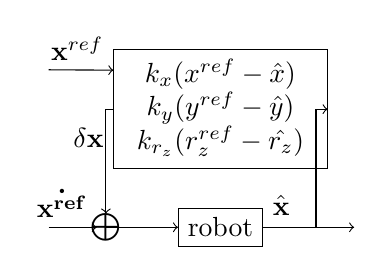
\begin{tikzpicture}[x=.40\textwidth,y=2.5cm]

      \path node (plus) at (-0.45,0) [shape=rectangle,draw,color=white]
            {\color{black} $\bigoplus$};

      \path node (robot) at (-0.15,0)
            [shape=rectangle,draw,label=3:$\hat{\mathbf{x}}$] {robot};

      \path node (errorcomp) at (-0.15,0.6)
            [shape=rectangle,draw,label=185:$\mathbf{\delta \mathbf{x}}$]
            {$\begin{array}{c}
                k_x (x^{ref} - \hat{x})\\
                k_y (y^{ref} - \hat{y})\\
                k_{r_z} (r_z^{ref} - \hat{r_z})\end{array}$};

      \draw[-] (-0.45,0.6) -- (errorcomp.west);
      \draw[->] (-0.45,0.6) -- (-0.45,0.07);

      \draw[->] (0.1,0.6) -- (errorcomp.east);
      \draw[-] (0.1,0.6) -- (0.1,0.);
      \draw[->] (robot.east) -- (0.2,0.);

      \draw[->] (-0.45,0.) -- (robot.west);

      \draw[->] (-0.6,0.) -- (-0.474,0.) node [above left]
           {$\mathbf{\dot{\mathbf{x}^{\text{ref}}}}$};

      \draw[->] (-0.6,0.8) -- (errorcomp.160) node [above left]
           {$\mathbf{x}^{\text{ref}}$};
    \end{tikzpicture}
  \end{center}
  \caption{Correction de trajectoire pour un robot type base
    mobile. $\mathbf{x}^{\text{ref}} = (x^{\text{ref}},
    y^{\text{ref}}, r_z^{\text{ref}})$, $\mathbf{\dot{x}^{\text{ref}}}
    = (\dot{x}^{\text{ref}}, \dot{y}^{\text{ref}},
    \dot{r_z}^{\text{ref}})$ et $\mathbf{\hat{x}} = (\hat{x}, \hat{y},
    \hat{r_z})$ sont respectivement la position et vitesse du robot
    dans le plan et dans la réalité. La commande planifiée
    $\mathbf{\dot{x}}$ est corrigée en sommant $\delta \mathbf{x}$ une
    correction déterminée par l'erreur de positionnement d'un point de
    référence du robot entre le plan et la position donnée par le
    système de localisation. \label{fig:system}}
\end{figure}

Si l'on appliquait ce système à un robot humanoïde, il mettrait à jour
une trajectoire de référence, celle du centre de masse, par
exemple. Tant que le robot a au moins un pied au sol, le bassin est
contrôlable localement ce qui permet d'appliquer la correction en
modifiant la valeur de degrés de liberté de la jambe.


\paragraph{Stabilité de la trajectoire corrigée}


Contrairement aux robots mobiles, les trajectoires stables pour un
robot humanoïde sont peu nombreuses en proportion. Tout l'enjeu de la
génération d'une trajectoire pour un robot humanoïde est d'assurer sa
stabilité. Il faut donc vérifier que la correction de la trajectoire
initiale ne viendra pas compromettre cette stabilité. Comme nous
l'avons vu dans la section précédente, il faut corriger la trajectoire
sans faire sortir le ZMP du polygone support:

\begin{equation} \label{eq:zmp2}
  \mathbf{z} = \mathbf{x}  - \frac{z_c}{g} \ddot{\mathbf{x}}
\end{equation}

La linéarité de l'équation signifie que perturber le center masse par
une fonction \mbox{$\delta \mathbf{x}$} dépendant du temps perturbe le
ZMP de manière linéaire:

\begin{equation} \label{eq:zmpperturbation}
\begin{split}
  \mathbf{z'} &= (\mathbf{x} + \mathbf{\delta x}) - \frac{z_c}{g} .
  \frac{d^2 (\mathbf{x} + \mathbf{\delta x})}{d t^2}\\
  &= \mathbf{x} - \frac{z_c}{g} \ddot{\mathbf{x}} +
  \underbrace{\mathbf{\delta x} - \frac{z_c}{g} \ddot{\mathbf{\delta
        x}}}_{\text{perturbation induite}}
\end{split}
\end{equation}

En utilisant le modèle linéaire, il est possible d'étudier comment
modifier la trajectoire du centre de masse pour assurer l'équilibre de
la trajectoire.

De plus, il est possible d'effectuer le raisonnement en utilisant le
modèle linéaire sur la perturbation uniquement. On peut donc utiliser
un algorithme de génération de mouvement hors-ligne coûteux et
raffiner le mouvement en temps réel via la méthode proposée dans la
section suivante. L'intérêt est de pouvoir combiner à la fois des
trajectoires qui sont trop dynamiques pour pouvoir utiliser le modèle
linéaire tout en considérant localement que les équations sont
linéaires pour ajuster localement la trajectoire.


\paragraph{Singularités des trajectoires corrigées}


Dans la mesure où le bassin d'un robot humanoïde n'est que localement
actionnable, il est primordial de générer des corrections qui
n'introduisent pas de singularités durant le mouvement. Typiquement,
un écart trop important entre les points de contact et la trajectoire
du centre de masse -- souvent proche du bassin -- peut provoquer des
singularités. Il est donc nécessaire non seulement de corriger le
positionnement du bassin, mais également de déformer les points de
contact afin d'éviter les singularités. Dans le cas contraire, on
observerait une ``dérive'' du bassin qui s'éloignerait progressivement
des empreintes de pas planifiées.

Il apparaît donc clairement qu'une solution naïve inspirée de la
robotique mobile n'est pas une solution viable. Dès lors, corriger la
trajectoire d'un robot humanoïde pour pouvoir s'asservir sur un
capteur demande une approche originale qui sera détaillée dans la
section suivante. Le schéma de contrôle proposé tient compte de ces
deux problèmes afin de fournir une approche adaptée à la locomotion
bipède.

\section{Suivi de trajectoire pour la robotique humanoïde}\label{closedloop}


Cette section propose un contrôleur pour le suivi de trajectoire
boucle fermée pour les robots humanoïdes qui prend en compte leurs
particularités.

Suivre une trajectoire asservie consiste à exécuter une trajectoire
précalculée tout en s'assurant que les erreurs d'exécution sont bien
compensées. Un tel système se divise en quatre composants:

\begin{enumerate}
\item un générateur de trajectoire,
\item un système de localisation fournissant une estimation de la position du robot,
\item un système d'estimation de l'erreur calculant l'écart entre la
  position actuelle du robot et celle à laquelle il est censé se
  trouver,
\item et un composant générant une trajectoire mise à jour permettant
  de réduire l'écart constaté.
\end{enumerate}


Le générateur de trajectoires fournit deux données de référence: la
séquence d'empreintes de pas, c'est-à-dire un ensemble de $S_i$ tel
que \mbox{$0 \leq i \leq n^{\text{pas}}$} et une trajectoire du haut
du corps \mbox{$\gamma(t \in [t_{\text{min}}, t_{\text{max}}]) \in
  \mathcal{C}$}. Un avantage du schéma de contrôle proposé est que la
position des empreintes de pas peut être altéré pour s'assurer que la
trajectoire reste faisable. En partant d'une modification de la pile
de pas, on peut déformer la trajectoire du centre de masse pour
s'assurer que la trajectoire reste stable. Les trajectoires de
référence portent sur des points du corps du robot et ne contiennent
pas directement les valeurs articulaires. La pile de tâches a donc pour
tâche de résoudre la cinématique inverse en temps réel lors de la
résolution du problème d'optimisation.

Une itération de la boucle de contrôle est décrite par l'algorithme \ref{fig:control_loop} et peut être résumée aux étapes suivantes:

\begin{enumerate}
\item estimation de la position du robot,
\item calcule de l'erreur de positionnement \mbox{$\delta \mathbf{x}$},
\item filtrage de l'erreur calculée par un filtre passe-bas afin de
  borner la déformation maximum et absorber d'éventuelles erreurs de
  localisation,
\item recalculer les prochains pas de façon à absorber l'erreur de
  positionnement du robot,
\item vérifier si le prochain pas est réalisable,
\item regénérer des trajectoires continues pour les pieds, le ZMP et le centre de masse,
\item recalculer les valeurs articulaires via la pile de tâches
\end{enumerate}


\begin{algorithm}
  \begin{algorithmic}
    \REQUIRE {$\gamma$, $t_{\text{maintenant}}, t_{\text{prochain}}$}
    \ENSURE {$\gamma$, $t_{\text{maintenant}}, t_{\text{prochain}}$}
    \IF {$\gamma(t_{\text{maintenant}})$ est en double support \AND
      $t_{\text{maintenant}} \geq t_{\text{prochain}}$}
    \STATE estimer la position du robot $\mathbf{\hat{x}}$
    \STATE calculer l'erreur de positionnement $\delta \mathbf{x}$
    \STATE calculer la déformation $\delta \gamma$ permettant de
    corriger l'erreur de positionnement $\delta \mathbf{x}$
    \IF {la correction $\delta \gamma$ peut être appliquée}
    \STATE $\forall t \in [t_{\text{maintenant}}, t_{\text{max}}],
    \gamma(t) \leftarrow \gamma(t) \bigoplus \delta \gamma(t)$
    \STATE $t_{\text{prochain}} \leftarrow t_{\text{maintenant}} + 2 T_{\text{step}}$
    \ENDIF
    \ENDIF
    \STATE $\mathbf{q} \leftarrow \gamma(t_{\text{maintenant}})$
    \STATE $t_{\text{maintenant}} \leftarrow t_{\text{maintenant}} + \Delta t$
  \end{algorithmic}
  \caption{Boucle de contrôle au temps $t_{\text{maintenant}}$ réalisant
    un suivi de trajectoire boucle-fermée de la trajectoire $\gamma$
    (la prochaine correction sera appliquée au temps
    $t_{\text{prochain}}$). \label{fig:control_loop}}
\end{algorithm}

Tout d'abord, la position du robot $\hat{\mathbf{x}}$ est
déterminée. Une large littérature concernant la localisation robotique
existe \cite{08ijhr.stasse, 06humanoids.thompson} et les spécificités
de la localisation d'un robot humanoïde seront abordées dans le
prochain chapitre. Les limites habituelles de la localisation sont la
perte du suivi résultant dans l'absence de localisation pendant un
moment plus ou moins long ou bien la présence de bruit, voire de
valeurs aberrantes dans l'estimation fournie.

Deuxièmement, une erreur $\mathbf{\delta \mathbf{x}}$ est calculée en
comparant la position planifiée et la position estimée du corps de
référence. Un seuil est appliqué pour borner la correction pouvant
être appliquée. En pratique, ce filtrage permet de limiter l'influence
du bruit de localisation ainsi que les valeurs aberrantes lorsque la
localisation échoue.


\begin{figure}[ht!]
  \begin{center}
    \begin{tikzpicture}[x=.40\textwidth,y=2.5cm]
      \def\w{0.3}
      \def\h{0.35}

      \def\ws{0.05}
      \def\hs{0.2}

      \def\noisex{0.01}
      \def\noisey{0.3}

      \foreach \dy in {0., 1.}
               {
                 \draw[pattern=dots,rounded corners]
                 (0.,0.25+\dy) rectangle (0.+\w,0.25+\dy+\h);

                 \draw[rotate=-10,rounded corners]
                 (\noisex,0.25+\noisey + \dy) rectangle
                 (\noisex+\w,0.25+\noisey+\dy+\h);

                 % left step planned
                 \filldraw[pattern=north east lines] (
                 0. + 0.1   * \w,
                 0.5 + \dy + 0.225 * \h)
                 rectangle (
                 0. + 0.1   * \w + \ws,
                 0.5 + \dy + 0.225 * \h + \hs);

                 % right step planned
                 \filldraw[pattern=north east lines] (
                 0. + 0.75 * \w,
                 \dy + 0.225  * \h)
                 rectangle (
                 0. + 0.75  * \w + \ws,
                 \dy + 0.225 * \h + \hs);

                 % left step real
                 \draw[rotate=-10] (
                 \noisex + 0.1   * \w,
                 0.5 + \noisey + \dy + 0.225 * \h)
                 rectangle (
                 \noisex + 0.1   * \w + \ws,
                 0.5 + \noisey + \dy + 0.225 * \h + \hs);

                 % right step real
                 \draw[rotate=-10] (
                 \noisex + 0.75 * \w,
                 \noisey + \dy + 0.225  * \h)
                 rectangle (
                 \noisex + 0.75  * \w + \ws,
                 \noisey + \dy + 0.225 * \h + \hs);
               }

               \draw[smooth,-,thick]
               (0.75 * \w + \ws/2.,\h/2.) --
               (0.75 * \w + \ws/2.,1.+\h/2.)
               node[midway,left]
               {
                 $\gamma$
               };

               \draw[smooth,rounded corners=1ex,-,thick]
               (0.75 * \w + \ws/2. + 0.03,0.15+\h/2. + 0.15) --
               (0.75 * \w + \ws/2. + 0.03 + 0.03,0.15+\h/2. + 0.15 + 0.4) --
               (0.75 * \w + \ws/2.,1.+\h/2.)
               node[at start,right]
               {
                 $\gamma \bigoplus \delta \gamma$
               };

               \draw[smooth,rounded corners=1ex,<->,thick]
               (-0.02, 0.25+0.45) --
               (-0.03, 0.25+0.35) --
               (-0.02, 0.25+0.25)
               node[at start,left]
               {
                 $\Delta r_z$
               };

               \draw[smooth,rounded corners=1ex,<->,thick]
               (-0.02, 0.25+0.) --
               (-0.02, 0.25+0.15)
               node[midway,left]
               {
                 $\Delta x$
               };

               \draw[smooth,rounded corners=1ex,<->,thick]
               (0., 0.25-0.1) --
               (0.03, 0.25-0.1)
               node[midway,below]
               {
                 $\Delta y$
               };

               \path node (txt1) at (0.075+\w,0.25+0.)
                     [shape=rectangle,draw,color=white]
                     {\color{black} $\mathbf{x}$};

               \path node (txt1) at (0.08+\w,0.25+0.3)
                     [shape=rectangle,draw,color=white]
                     {\color{black} $\mathbf{\hat{x}}$};

    \end{tikzpicture}
  \end{center}
  \caption{Correction of the next step due to a position error. Dotted
    rectangles are the planned positions $\mathbf{x}$ of the robot
    waist and feet before and after the next step. Non-dotted
    rectangles corresponds to the robot localization
    $\mathbf{\hat{x}}$. Error w.r.t to axis X, Y and yaw rotation is
    \mbox{$(\Delta x, \Delta y, \Delta r_z) = \delta \mathbf{x}$,
      $\gamma$} the reference trajectory and $\delta \gamma$ the
    corrected trajectory reaching the planned
    step. \label{fig:footstepreplan}}
\end{figure}


Ensuite, la position du prochain pas est modifiée afin de compenser
l'erreur calculée. La figure \ref{fig:footstepreplan} illustre cette étape.


À partir de ce moment, il est possible de regénérer des trajectoires
pour les pieds et le centre de masse. Afind d'assurer la continuité de
la solution, la correction de la trajectoire est appliquée
progressivement durant les deux prochains pas. Pour finir, la
résolution des tâches calcule les nouvelles valeurs articulaires.


Avant de commencer une correction, un test est effectué pour
déterminer si une correction est possible au moment courant
$t_{\text{maintenant}}$. Une correction ne peut commencer que si le
robot est en double support et qu'aucune autre correction n'est en
cours de réalisation, c'est-à-dire \mbox{$t_{\text{maintenant}} \geq
  t_{\text{prochain}}$}. En effet, corriger de nouveau alors que la
correction précédente n'est pas totalement appliquée conduit à
corriger une partie de l'erreur de localisation plusieurs fois.


Les travaux précédents tel que \cite{04humanoids.harada,
  07icra.morisawa} ont pour but de permettre des changements soudains
dans la trajectoire des pieds -- et donc du centre de masse -- tout en
préservant l'équilibre du robot. Le schéma de contrôle proposé a pour
but, au contraire, de rester aussi proche que possible du plan initial
et ne sert donc pas le même objectif.


\paragraph{Estimation de l'erreur de positionnement}

Nous faisons l'hypothèse ici que le système fournit
\mbox{$\hat{\mathbf{x}} \in \text{SE}(2)$}, une estimation de la
position actuelle du robot.

Si $\mathbf{x} \in \text{SE}(2)$ est la position planifiée du robot et
$\hat{\mathbf{x}} \in \text{SE}(2)$ sa localisation estimée, l'erreur
est définie par:

\begin{equation}\label{eq:errorpos}
  \mathbf{\delta x} = \mathbf{x} . \hat{\mathbf{x}}^{-1}
\end{equation}

Dans l'équation précédente, $\mathbf{\delta x}(t)$ peut être
interprétée comme la position du robot planifiée par rapport à la
position du robot estimée. Le délai induit par le système de
localisation fait que l'estimation du robot doit être comparée à la
position dans le plan au même moment. On obtient alors une erreur sur
le positionnement à un moment du passé, mais qui peut être utilisé
sans problème. On peut raisonnablement estimer que l'erreur de
positionnement croît avec le temps et qu'on ne compensera donc
l'erreur qu'en partie, mais on évitera une trop grande divergence
entre le plan et la réalité. On estime également que l'erreur de
positionnement initial est toujours nul:

\begin{equation}\label{eq:errorpos_prop}
\delta \mathbf{x}(t_{\text{min}}) = 0
\end{equation}

\paragraph{Modification de la séquence de pas}

Étant donné une erreur de localisation d'un corps de référence, le
bassin en général, il est possible d'altérer la pile de pas restante à
exécuter pour absorber cette erreur.

L'objectif de cette étape est donc de faire en sorte de déformer la
suite du mouvement pour que le robot pose ses pieds aux endroits
planifiés.

Les empreintes de pas sont \mbox{$S \in
  \text{SE}(2)^{n^\text{pas}}$}. Considérons $\mathbf{\delta {x}}$,
l'erreur de positionnement courant, et \mbox{$S^{\text{futur}} \subset
  S$} les pas restant encore à réaliser. Les empreintes de pas futures
seront déformées en utilisant la relation suivante:

\begin{equation}\label{eq:footstepmodif}
  \forall s \in S^{\text{future}}, s \gets \mathbf{\delta {x}} . s
\end{equation}

\paragraph{Modification des trajectoires de référence}

De nouvelles positions pour les points d'appui ont été calculées. Il
est donc désormais nécessaire de modifier la trajectoire des deux
pieds ainsi que du centre de masse pour pouvoir corriger le
positionnement des deux pieds dans le futur.

La correction de la trajectoire du centre de masse est calculée en
utilisant le modèle simplifié introduit précédemment FIXME. De fait,
aucune hypothèse n'est faite pour réaliser la correction et en
particulier le générateur de trajectoire n'est jamais mis à
contribution pour regénérer les trajectoires de référence. C'est là la
différence majeure qui différencie cette approche de la
replanification. Ces approches se fondent sur un recalcul complet des
trajectoires de marche régulère en changeant la position du robot à
partir de l'estimation de sa position. Si cette approche est adaptée
lorsque la planification a un coût peu important, comme sur les bases
mobiles, elle ne l'est pas dans le cadre de la robotique humanoïde où
les algorithmes de génération de mouvement ont un coût
important. L'hypothèse proposée ici est qu'utiliser un modèle
linéarisé pour réaliser de petites corrections perturbe peu la
trajectoire et ne compromet pas la qualité du résultat de manière
significative.


Supposons que le modèle linéaire a été utilisé pour générer le
mouvement, la résolution analytique nous donne l'équation suivante,
déjà détaillée dans la section précédente:

\begin{equation} \label{eq:zmpsol}
  \mathbf{x}(t) = \cosh(\sqrt{\frac{g}{z_G}}.t) . \mathbf{V} + \sinh(\sqrt{\frac{g}{z_G}}.t) . \mathbf{W} + \mathbf{r}(t)
\end{equation}


Dans la section précédente, nous avons déplacé les pas
futurs. L'objectif est donc de raccrocher la trajectoire de ZMP à la
nouvelle pile de pas. Cependant, contrairement aux pas qui sont des
données discrètes, les trajectoires doivent être raccordées
continument. Pour ce faire, nous avons choisi un polynôme de degré
trois à valeurs réelles auquel quatre contraintes ont été imposées,
voire Fig. \ref{fig:transition}. Ce polynôme est dénoté
$\Delta_\alpha(t)$ où $\alpha$ est la valeur du polynôme à $t=T$. Les
contraintes sont donc:

\begin{figure}[ht!]
  \begin{center}

    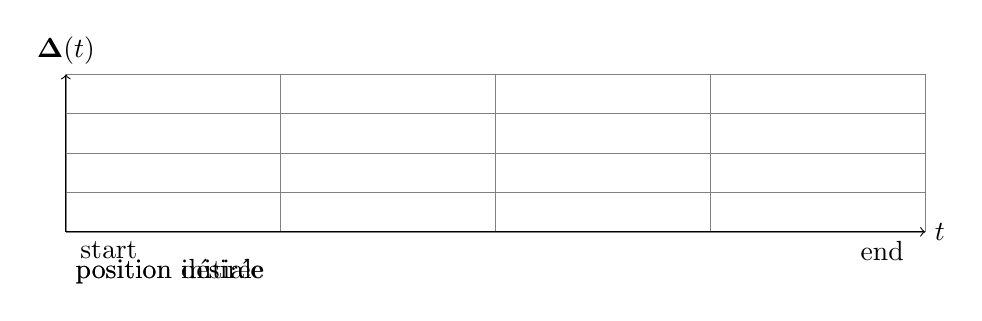
\begin{tikzpicture}[x=.9\textwidth]
      \def\xmin{0.}
      \def\xmax{1.}
      \def\ymin{0.5}
      \def\ymax{2.5}

      % grid
      \draw[style=help lines, ystep=.5, xstep=.25] (\xmin,\ymin) grid
      (\xmax,\ymax);

      % axes
      \draw[->] (\xmin,\ymin) -- (\xmax,\ymin) node[right] {$t$};
      \draw[->] (\xmin,\ymin) -- (\xmin,\ymax) node[above]
           {$\mathbf{\Delta}(t)$};

      % xticks and yticks
      \node at (0.05, \ymin) [below] {start};
      \node at (0.95, \ymin) [below] {end};

      \draw[color=black,domain=\xmin:\xmax] plot[id=cur] function{1}
      node [right] {position initiale};

      \draw[color=black, domain=\xmin:\xmax] plot[id=des]
      function{2} node [right] {position désirée};

      \draw[color=black, domain=\xmin:\xmax] plot[id=trans]
      function{-2. * x * x * x + 3 * x * x + 1} node [below] {};

    \end{tikzpicture}
  \end{center}
  \caption{Courbe polynomiale $\mathbf{\Delta}(t)$ réalisant une
    transition continue lors de la mise à jour des
    trajectoires. \label{fig:transition}}
\end{figure}

\begin{enumerate}
\item $\forall t \leq 0, \Delta_\alpha(t) = 0$
\item $\forall t \leq 0, \dot{\Delta_\alpha}(t) = 0$
\item $\forall t \geq T, \Delta_\alpha(t) = \alpha$
\item $\forall t \geq T, \dot{\Delta_\alpha}(t) = 0$
\end{enumerate}

En pratique, $T$ représente la durée d'un pas. Ce polynôme sera
utilisé pour fournir des transitions continues, composante par
composante, aux différentes trajectoires de référence. Qui plus est,
les quatre contraintes contraignent totalement ce polynôme de degré
trois pour lequel il existe donc une unique solution sur l'intervalle
$[0,T]$. Les valeurs extérieures étant définies par les contraintes
directement. On notera enfin que même si ce polynôme est à valeur dans
$\mathbb{R}$ quand $\alpha \in \mathbb{R}$, on peut aussi bien le
définir sur $\mathbb{R}^n$, $n \in \mathbb{N}^+$ à condition que
$\alpha \in \mathbb{R}^n$.


Une fois ce polynôme défini, il est possible de rattacher la
trajectoire de ZMP en sommant à la trajectoire de référence du ZMP, le
polynôme $\mathbf{\Delta}_{\mathbf{\delta {x}}}(t)$. La résolution du
système est alors le suivant:

\begin{equation} \label{eq:zmpsolcor}
  \bar{\mathbf{c}}(t) = \cosh(\sqrt{\frac{g}{z_c}}.t) . \mathbf{V} +
  \sinh(\sqrt{\frac{g}{z_c}}.t) . \mathbf{W} + \mathbf{r}(t) + \mathbf{\Delta}_{\mathbf{\delta {x}}}(t)
\end{equation}

En effet, la substitution de variable $\mathbf{r}(t)$ par
$\mathbf{r}(t) + \mathbf{\Delta}_{\mathbf{\delta {x}}}(t)$ ne change
que le second membre de l'équation homogène et ne perturbe pas la
solution générale.

L'équation précédente réalise une correction à $t=0$. Évidemment, ce
n'est pas toujours le cas. En pratique, une correction est commencée
tous les deux pas, lorsque le robot est en double support. Si l'on a
corrigé trois fois la trajectoire à $t_1$, $t_2$ et $t_3$, la
trajectoire est alors:

\begin{equation} \label{eq:zmpsolcor2}
  \bar{\mathbf{c}}(t) = \cosh(\sqrt{\frac{g}{z_c}}.t) . \mathbf{V} +
  \sinh(\sqrt{\frac{g}{z_c}}.t) . \mathbf{W} + \mathbf{r}(t) +
  \mathbf{\Delta}_{\mathbf{\delta {x}}(t_1)}(t-t_1) +
  \mathbf{\Delta}_{\mathbf{\delta {x}}(t_2)}(t-t_2) +
  \mathbf{\Delta}_{\mathbf{\delta {x}}(t_3)}(t-t_3)
\end{equation}

$\mathbf{\delta {x}}(t)$ étant l'erreur de localisation au temps
$t$. Plus généralement, on obtient donc la relation suivante où
$t_{\text{correction}}$ est l'ensemble des temps où une correction a
été appliquée:

\begin{equation} \label{eq:zmpsolcor2}
  \bar{\mathbf{c}}(t) = \cosh(\sqrt{\frac{g}{z_c}}.t) . \mathbf{V} +
  \sinh(\sqrt{\frac{g}{z_c}}.t) . \mathbf{W} + \mathbf{r}(t) +
  \sum_{t_i \in t_{\text{correction}}} \mathbf{\Delta}_{\mathbf{\delta {x}}(t_i)}(t-t_i)
\end{equation}

\begin{figure}[ht!]
  \begin{center}
    \begin{tikzpicture}[x=.9\textwidth]
      \begin{axis}[
          xlabel=temps ($\mathrm{s}$),
          ylabel= position en $x$ ($\mathrm{m}$),
          no markers
          ]

        \addplot[
          mark=x,
          red
        ] table[
          x expr=(\thisrowno{0}-0)*0.005
        ] {dat/feet_follower_feet-follower-com.dat};
        \label{com}
        \addplot[
          mark=x,
          red,
          line width=1.25pt
        ] table[
          x expr=(\thisrowno{0}-0)*0.005,
          y expr=\thisrowno{1}-0.
        ] {dat/feet_follower_correction-com.dat};
        \label{comcorr}

        \addplot[
          mark=*,
          blue,
          loosely dashed
        ] table[
          x index=0,
          y index=4,
          x expr=(\thisrowno{0}-0)*0.005
        ] {dat/feet_follower_feet-follower-left-ankle.dat};
        \label{lf}

        \addplot[
          mark=*,
          blue,
          line width=1.25pt,
          loosely dashed
        ] table[
          x index=0,
          y index=4,
          x expr=(\thisrowno{0}-0)*0.005,
          y expr=\thisrowno{4}-0.
        ] {dat/feet_follower_correction-left-ankle.dat};
        \label{lfcorr}

        \addplot[
          mark=triangle*,
          green,
          dashed
        ] table[
          x index=0,
          y index=4,
          x expr=(\thisrowno{0}-0)*0.005
        ] {dat/feet_follower_feet-follower-right-ankle.dat};
        \label{rf}

        \addplot[
          mark=triangle*,
          green,
          dashed,
          line width=1.25pt
        ] table[
          x index=0,
          y index=4,
          x expr=(\thisrowno{0}-0)*0.005,
          y expr=\thisrowno{4}-0.
        ] {dat/feet_follower_correction-right-ankle.dat};
        \label{rfcorr}
      \end{axis}
    \end{tikzpicture}
  \end{center}
  \caption{Évolution, pendante deux pas, de la position en $x$ du
    centre de masse (\ref{com}), du pied gauche (\ref{lf}) et du pied
    droit (\ref{rf}). La courbe en gras illustre un pas de $0.3
    \mathrm{m}$ en avant. Les courbes en pointillé illustre la
    position du centre de masse (\ref{comcorr}), pied
    gauche (\ref{lfcorr}) et pied droit (\ref{rfcorr}) après un pas de
    $0.05 \mathrm{m}$ en avant, soit une correction de $0.02
    \mathrm{m}$. \label{fig:traj}}
\end{figure}


L'équation précédente définit comment déformer la trajectoire du
centre de masse. La déformation de la trajectoire des pieds est
directe, en utilisant le polynôme $\mathbf{\Delta}$ pour assurer que
les trajectoires de chaque pas terminent bien à la position prévue
dans la pile de pas modifiée. Cependant, un dernier point reste à
traiter: la synchronisation temporelle de la correction du pied
gauche, droit et du centre de masse. Elle est réalisée en deux temps:
le premier pied qui bouge et le centre de masse sont d'abord corrigés
puis le deuxième pied est ensuite corrigé pendant sa phase de
vol. Évidemment, il n'est pas possible de déplacer un pied au sol d'où
la nécessité d'utiliser deux pas pour corriger complètement la
trajectoire. On remarquera que la modification synchronisée de la
trajectoire du centre de masse et de la trajectoire du premier pas
permet d'assurer que le ZMP reste à tout moment dans le polygone
support. En effet, la trajectoire du ZMP étant déformée d'autant que
la trajectoire du centre de masse, ce dernier termine à une position
équivalente à la fin du pas, relativement au pas aillant effectué le
mouvement. La Figure \ref{fig:traj} illustre ces trois corrections
synchronisées.


\paragraph{Filtrage de l'erreur et faisabilité du prochain pas}


La correction ne compromet pas la stabilité du robot. Cependant, la
correction n'est pas toujours réalisable, car l'espace d'accessibilité
du pied est fini à la fois à cause de sa géométrie et d'éventuelles
autocollisions pouvant se produire -- une jambe pouvant entrer en
collision avec la seconde --. De ce fait, il est important de borner
les corrections pour éviter les autocollisions.


Les hypothèses de travail sont que la trajectoire de référence est
elle-même stable et sans collision. Par conséquent, l'objectif est
alors de savoir quelles sont les bornes à partir desquelles il n'est
plus possible de corriger le mouvement.


La première étape a été de déterminer une enveloppe dans laquelle les
corrections sont réalisables géométriquement parlant -- la cinématique
inverse des jambes est soluble --. La perturbation latérale maximum
est de $\pm 0.04 \mathrm{m}$, la perturbation frontale, quant à elle,
est de $\pm 0.05 \mathrm{m}$ et la perturbation angulaire maximum est
de $\pm 0.1 \mathrm{rad}$ tous les deux pas. Ces valeurs correspondent
à une borne sur la valeur $\mathbf{\delta {x}}$, l'erreur de
positionnement du robot.


\begin{figure}[ht!]
  \begin{center}
    \begin{tikzpicture}[x=.40\textwidth,y=2.5cm]
      \def\w{0.3}
      \def\h{0.25}

      \def\ws{0.05}
      \def\hs{0.2}

      \def\noisex{0.01}
      \def\noisey{0.3}

      % left step planned
      \filldraw[pattern=north east lines] (
      0. + 0.1   * \w,
      0. + 0.225 * \h)
      rectangle (
      0. + 0.1   * \w + \ws,
      0. + 0.225 * \h + \hs);
      \filldraw[pattern=north east lines] (
      0. + 0.1   * \w,
      1. + 0.225 * \h)
      rectangle (
      0. + 0.1   * \w + \ws,
      1. + 0.225 * \h + \hs);


      % right step planned
      \filldraw[pattern=north east lines] (
      0. + 0.75 * \w,
      0. + 0.225  * \h)
      rectangle (
      0. + 0.75  * \w + \ws,
      0. + 0.225 * \h + \hs);

      \filldraw[pattern=north east lines] (
      0. + 0.75 * \w,
      1. + 0.225  * \h)
      rectangle (
      0. + 0.75  * \w + \ws,
      1. + 0.225 * \h + \hs);


      \foreach \dy in {0., 1.}
               {
                 \draw[pattern=dots,rounded corners] (0.,\dy)
                 rectangle (0.+\w,\dy+\h);
               }

               % valid 1
               \filldraw[pattern=north east lines,rotate=-10] (
               0. + 0.75 * \w,
               1. + 0.225  * \h)
               rectangle (
               0. + 0.75  * \w + \ws,
               1. + 0.225 * \h + \hs);

               % valid 2
               \filldraw[pattern=north east lines,rotate=10] (
               0. + 0.75 * \w + 0.1,
               1. + 0.225  * \h)
               rectangle (
               0. + 0.75  * \w + \ws + 0.1,
               1. + 0.225 * \h + \hs);


               % invalid 1
               \filldraw[color=black,rotate=10] (
               0. + 0.75 * \w,
               1. + 0.225  * \h)
               rectangle (
               0. + 0.75  * \w + \ws,
               1. + 0.225 * \h + \hs);

               % invalid 2
               \filldraw[color=black,rotate=-10] (
               0. + 0.75 * \w - 0.12,
               1. + 0.225  * \h)
               rectangle (
               0. + 0.75  * \w + \ws - 0.12,
               1. + 0.225 * \h + \hs);

               % arrow
               \draw[smooth,-,thick]
               (0.75 * \w + \ws/2.,\h/2.) --
               (0.75 * \w + \ws/2.,1.+\h/2.)
               node[midway,left]
               {
                 $\gamma$
               };

               \path node (txt1) at (0.375+\w,0.2)
                     [shape=rectangle,draw,color=white]
                     {\color{black} position actuelle};

               \path node (txt1) at (0.375+\w,1.3)
                     [shape=rectangle,draw,color=white]
                     {\color{black} position après le pas};
    \end{tikzpicture}
  \end{center}
  \caption{Validation du pas recalculé. La position du bassin est
    symbolisée par le rectangle en pointillé. Les pas valides sont
    hachurés tandis que les pas invalides sont de couleur noire.
    \label{fig:stepvalid}}
\end{figure}


\begin{figure}
  \begin{center}
    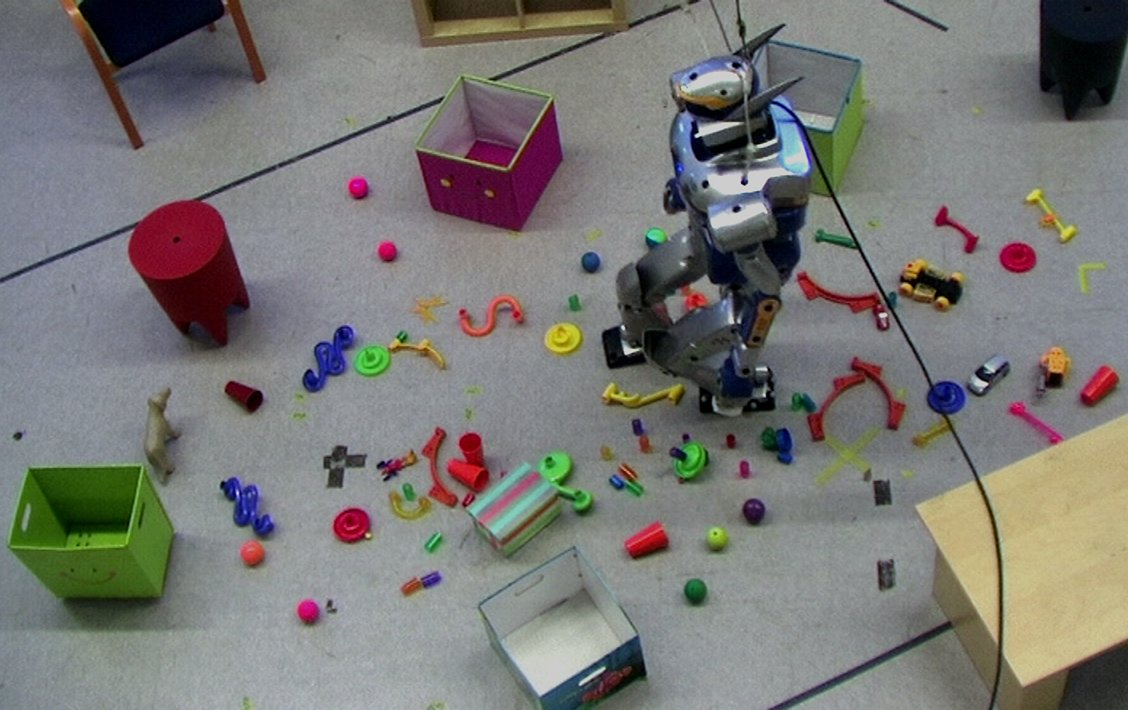
\includegraphics[width=\textwidth]{src/chap2-suivi-trajectoire/demo.jpg}
  \end{center}
  \caption{HRP-2 marchant dans un environnement extrêmement encombré
    tout en évitant des obstacles. La précision finale est atteinte
    avec une précision de $\pm 3\mathrm{cm}$. L'erreur finale est la
    conséquence du bruit impactant l'estimation de la position du
    robot ainsi que de la dérive accumulée sur la fin de la
    trajectoire qu'il n'est pas possible de corriger, faute de
    temps. \label{fig:scenario}}
\end{figure}


Ensuite, le nouveau pas est validé. La décision se fonde sur le
raisonnement géométrique suivant: le pied d'HRP-2 ne peut pas entre en
collision avec lui-même. Par conséquent, les seules collisions
possibles sont qu'un pied entre en collision avec le second. De ce
fait, si l'on ignore les configurations rares du type, ``le robot
croise les jambes en marchant'', possibles, mais aux limites des
capacités articulaires des jambes, on peut tenir le raisonnement
suivant: on peut toujours déplacer un pas du pied gauche vers la
gauche sans entrer en collision et un pas du pied droit vers la droite
sans entraîner de collision. De même on peut toujours faire tourner la
structure vers l'extérieur sans provoquer de collisions. L'heuristique
suivante est donc utilisée pour valider les pas. Elle est, évidemment,
sous-optimale, mais est sûre et a un coût en temps de calcul quasi
nul.


Si la correction est invalidée pour une des deux raisons précédemment
décrites, elle est alors abandonnée. À la prochaine phase de double
support, une nouvelle correction sera calculée et une nouvelle phase
de validation sera tentée. Dans la mesure où l'erreur de
positionnement croît lentement, il y a alors deux cas:
\begin{itemize}
\item Dans le premier, le signe de l'erreur de positionnement
  $\mathbf{\delta {x}}$ a changé, ce qui signifie que l'erreur de
  localisation était faible et qu'il n'était pas critique de la
  corrige maintenant,
\item Dans le second, le signe de l'erreur reste constant et il sera
  possible de corriger l'erreur, car la direction dans laquelle la
  correction est possible s'inverse en passant d'un pas avec le pied
  gauche à un pas avec le pied droit.
\end{itemize}

Ce système empirique a été validé avec succès sur le robot HRP-2. Un
objectif pour le futur est de remplacer cette heuristique par une
validation complète de la trajectoire de pas modifiée. Une stratégie
telle que celle décrite dans \cite{10icra.perrin} pourrait alors être
envisagée.

\section{Résultats expérimentaux}\label{exp}


La méthode proposée a été validée sur la plate-forme HRP-2 grâce au
scénario suivant: le robot doit naviguer dans un environnement
particulièrement contraint tout en enjambant des obstacles. La
longueur de la trajectoire est approximativement de $2.5\mathrm{m}$ et
est exécutée en environ $40\mathrm{s}$.


Ce scénario démontre que l'utilisation de ce schéma de contrôle permet
une navigation fiable. Le robot atteint l'objectif fixé avec une
précision de quelques centimètres tandis que le positionnement final
en utilisant un schéma de contrôle en boucle ouverte a une erreur
d'environ un mètre. De plus, ce schéma de contrôle est robuste aux
pertes de suivi et à des estimations peu précises par le système de
localisation. En effet, l'expérience s'appuie sur un système de
capture de mouvement pour localiser le robot. Ces derniers sont
extrêmement précis -- précision au millimètre dans les cas favorables
-- mais nécessitent un environnement dégagé ce qui n'est pas le cas
ici. Les marqueurs posés sur le pied sont parfois occlus par les
obstacles ce qui fait varier la précision durant le mouvement. Ce
comportement ne perturbe pas le schéma de correction qui peut
atteindre la position finale sans problème.


La vidéo de l'expérience est disponible sur internet:
\mbox{\url{http://youtu.be/cUZ0nNiPs70}}. La figure \ref{fig:scenario}
fournit un aperçu de l'expérience réalisée. Le robot part de la droite
et marche au travers des obstacles jusqu'à arriver à son but, sur la
partie gauche de l'image.

Dans ce contexte, la précision atteinte est de $\pm 2
\mathrm{cm}$. Cette trajectoire a été jouée cinq fois consécutivement
sans donner lieu à une collision avec un obstacle ou à une
autocollision. En utilisant un mouvement réalisant de plus petits pas,
la précision peut atteindre $1 \mathrm{cm}$. Les petits pas
nécessitent une accélération moindre du haut du corps et les effets
dynamiques mal modélisés par le modèle linéaire se font moins
ressentir, il en découle une erreur de positionnement des empreintes
de pas plus faible. L'algorithme de correction pour sa part dispose de
davantage de pas pour pouvoir réaliser des corrections. Ces deux
facteurs jouant pour améliorer la précision du suivi de trajectoire.


\section{Conclusion}\label{conclusion}


Cette section est divisée en deux et sert deux objectifs distincts. La
première partie est une introduction à la robotique humanoïde et
explique, en partant des relations fondamentales de la physique,
certains résultats récents de la littérature afin de fournir tous les
outils permettant de réaliser une tâche de locomotion pour un robot
humanoïde. Les robots humanoïdes alliant à la fois sous-actionnement
et redondance nécessitent des stratégies adaptées afin de pouvoir
générer des mouvements dans un temps raisonnable. En effet, le
problème en robotique humanoïde n'a jamais été de prévoir le mouvement
et la dynamique de corps dont les mouvements relatifs sont
contraints. Ces équations fondamentales de la physique sont connues
depuis longtemps. Le véritable enjeu est de trouver des modèles
calculatoires adaptés permettant un compromis idéal entre réalisme,
expressivité et réactivité. Différents outils de l'État de l'Art ont
été détaillé et sont assemblés pour former une plate-forme robotique
cohérente. La seconde partie propose un contrôleur pour le suivi de
trajectoire boucle fermée afin d'autoriser la navigation de précision
pour le robot humanoïde HRP-2. Cette section montre la barrière à
franchir pour passer d'une trajectoire simulée qui semble réalisable à
une application robotique fonctionnelle où la réalité physique et
l'incertitude d'exécution inhérente à la robotique réelle jouent un
rôle prépondérant. Nous avons essayé de montrer que des mouvements
complexes nécessitent des algorithmes complexes qui seront difficiles,
même à terme, à passer dans les contrôleurs temps réels des robots. De
ce fait, si l'on veut pouvoir dépasser la simple marche dans un sol
plan, il faudra sans doute passer par des stratégies d'adaptation
locales et réactives du plan plutôt que par une replanification
globale, ce que les approches récentes tendent à réaliser.
